\subsection{线性群中的指数映射}

命题 17. 设 \(\Delta\) 是由 \(z\in \mathbf{C}\) 满足 \(-\pi < \mathcal{I}(z) < \pi\) 所成的集合，而 \(\Delta'\) 是由 \(z\in \mathbf{C}\) 不是实数 \(\leqslant 0\) 所成的集合。设 \(E\) 是 \(\mathbf{C}\) 上的完备可赋范空间，且 \(A\)（分别地，\(A'\)）是由 \(x\in \mathcal{L}(E)\) 且其谱 \(\mathrm{Sp}(x)\) 包含于 \(\Delta\)（分别地，\(\Delta'\)）的元素构成的集合。则 \(A\)（分别地，\(A'\)）是 \(\mathcal{L}(E)\)（分别地，\(\mathbf{GL}(E)\)）的开子集，且映射 \(\exp: A\to A'\) 和 \(\log: A'\to A\)（谱理论，第 I 章，§4，第 9 号）是解析流形的互逆同构。

这由谱理论，第 I 章，§ 4，命题 10 和第 9 号得到。

定理 6. 设 E 是实或复 Hilbert 空间，U 是 E 的酉群。

\begin{enumerate}
\def\labelenumi{(\roman{enumi})}
\item
  \(\mathbf{H}\) 是 \(\mathcal{L}(\mathbf{E})\) 中厄米元素的集合；按实赋范空间结构，它是 \(\mathcal{L}(\mathbf{E})\) 的闭向量子空间，并具有拓扑补空间。
\item
  \(\mathbf{H}'\) 中满足 \(\geqslant 0\) 的元素的集合 \(\mathbf{GL}(\mathbf{E})\) 是 \(\mathbf{GL}(\mathbf{E})\) 的实解析子流形。
\item
  映射 exp 在 H 上的限制是从 H 到 H' 的实解析流形同构。
\item
  从 \((h,u)\mapsto (\exp h)u\) 到 \(\mathbf{H}\times \mathbf{U}\) 的映射 \(\mathbf{GL}(\mathbf{E})\) 是实解析流形同构。
\end{enumerate}

回忆，若 \(x \in \mathcal{L}(\mathrm{E})\)，则 \(x^*\)\(x\) 表示 x 的伴随。令 \(\mathrm{H}_1\) 为满足 \(x \in \mathcal{L}(\mathrm{E})\) 的 \(x^* = -x\) 的集合。公式 \(x = \frac{1}{2}(x + x^*) + \frac{1}{2}(x - x^*)\) 说明，按其实赋范空间结构，\(\mathcal{L}(\mathrm{E})\) 是 \(\mathrm{H}\) 与 \(\mathrm{H}_1\) 的拓扑直和，从而得到 (i)。

假设 \(\mathbf{K} = \mathbf{C}\)。在命题 17 的记号下，\(\mathrm{H}'\) 是满足 \(h \in \mathrm{H} \cap \Delta'\) 的 \(\mathrm{Sp} h \subset \mathbf{R}_{+}^{*}\) 的集合。由于 \(\exp(\mathbf{R}) = \mathbf{R}_{+}^{*}\)，(ii) 和 (iii) 由命题 17 以及谱理论，第 I 章，§4，命题 8 和 §6，第 5 号得到。从 \((h, u) \mapsto y = (\exp h)u\) 到 \(\mathrm{H} \times \mathrm{U}\) 的映射 \(\mathbf{GL}(\mathrm{E})\) 是双射，这是谱理论，第 I 章，§6，命题 15 的结论。由上可知它是实解析的。映射 \(y \mapsto h = \frac{1}{2} \log(yy^*)\) 是实解析的，因而映射 \(y \mapsto u = (\exp h)^{-1}y\) 也是实解析的。故得 (iv)。

假设 \(\mathbf{K} = \mathbf{R}\)。令 \(\hat{\mathbf{E}}\) 为 E 的复化 Hilbert 空间，令 J 为将 \(\xi + i\eta \mapsto \xi - i\eta\) 的映射（其中 \(\xi, \eta\) 属于 E），它从 \(\hat{\mathbf{E}}\) 到 \(\hat{\mathbf{E}}\)。令 \(\tilde{\mathbf{H}}, \tilde{\mathbf{H}}', \tilde{\mathbf{U}}\) 表示对 \(\hat{\mathbf{E}}\) 定义的集合，正如 H、H'、U 对 E 定义的那样。于是 H（分别地，H'、U）可与满足 \(x \in \tilde{\mathbf{H}}\) 的 \(\tilde{\mathbf{H}}'\)（分别地，\(\tilde{\mathbf{U}}\)、\(\mathrm{JxJ}^{-1} = x\)）的集合相识别。性质 (ii)、(iii) 和 (iv) 随即由 (i) 及复情形中的相应性质容易得到。

命题 18. 设 E 是 C 上的完备可赋范空间，\(v \in \mathcal{L}(E)\)，且 g = exp v。假定 \(\operatorname{Sp}(v)\) 不包含形如 \(2i\pi n\) 的点，其中 \(n \in Z - \{0\}\)。则对所有 \(x \in E\)，条件 vx = 0 与 gx = x 等价。

这由第 4 号的引理 2 应用于函数 \(z \mapsto e^z - 1\) 得到。

推论 1. 设 E 是 C 上的完备可赋范空间，F 是从 \(\mathbf{E}^n\) 到 E 的连续 n-线性映射空间。对所有 \(v \in \mathcal{L}(\mathbf{E})\)，令 \(\sigma(v)\) 为由下式定义的 \(\mathcal{L}(\mathbf{F})\) 中的元素：

\[
(\sigma (v) f) (x _ {1}, \dots , x _ {n}) = v (f (x _ {1}, \dots , x _ {n})) - \sum_ {i = 1} ^ {n} f (x _ {1}, \dots , v x _ {i}, \dots , x _ {n}).
\]

对所有 \(g \in \mathbf{GL}(\mathbf{E})\) ，令 \(\rho(g)\) 为由下式定义的 \(\mathbf{GL}(\mathbf{F})\) 中的元素：

\[
(\rho (g) f) (x _ {1}, \dots , x _ {n}) = g (f (g ^ {- 1} x _ {1}, \dots , g ^ {- 1} x _ {n})).
\]

设 \(u \in \mathcal{L}(\mathrm{E})\) 使得每个 \(z \in \operatorname{Sp} u\) 都满足 \(|\mathcal{I}(z)| < \frac{2\pi}{n + 1}\)。则对所有 \(f \in \mathrm{F}\)，条件 \(\sigma(u)f = 0\) 与 \(\rho(\exp u)f = f\) 等价。

\(L(\rho) = \sigma (\S 3, \text{no. } 11, \text{命题 41 的推论 1}) \text{从而}\)

\[
\rho (\exp u) = \exp \sigma (u)
\]

（第 4 号，命题 10 的推论 3）。由命题 18 可知，只需证明 \(\operatorname{Sp} \sigma(u)\) 不与 \(2i\pi(\mathbf{Z} - \{0\})\) 相交。但这由下述引理得到：

引理 6. 若 \(v \in \mathcal{L}(\mathrm{E})\)，则 \(\operatorname{Sp} \sigma(v) \subset \operatorname{Sp} v + \operatorname{Sp} v + \cdots + \operatorname{Sp} v\)，其中和式含有 \(n + 1\) 项。

对所有 \(v_{0}, v_{1}, \ldots, v_{n}\)，我们通过下式定义 \(\mathcal{L}(\mathrm{F})\) 中的元素 \(f \in \mathrm{F}\)：

\[
\begin{array}{l} (v _ {0} f) (x _ {1}, \dots , x _ {n}) = v (f (x _ {1}, \dots , x _ {n})) \\ (v _ {i} f) (x _ {1}, \dots , x _ {n}) = - f (x _ {1}, \dots , v x _ {i}, \dots , x _ {n}) \quad \text { for } 1 \leqslant i \leqslant n. \end{array}
\]

于是 \(\sigma(v) = \sum_{i=0}^{n} v_i\)，且各 \(v_i\) 两两可交换。令 A 为由 \(\mathcal{L}(F)\) 生成的 \(v_i\) 的闭子代数；它是交换的（

谱理论，第 I 章，§ 1，第 4 号），且 \(\mathrm{Sp}_{\mathcal{L}(\mathbb{F})}v' = \mathrm{Sp}_A v' \subset \sum_{i=0}^{n} \mathrm{Sp} v_i\)（谱理论，第 I 章，§ 3，命题 3 (ii)）。现在，若 \(\lambda \in \mathbf{C}\) 使得 \(v - \lambda\) 可逆，则显然 \(v_i - \lambda_i\) 可逆，从而对所有 \(\mathrm{Sp} v_i \subset \mathrm{Sp} v\)，\(i\)。

推论 2. 设 \(\mathbf{E}\) 是 \(\mathbf{C}\) 上的完备可赋范代数，且 \(w \in \mathcal{L}(\mathbf{E})\)。假定每个 \(z \in \operatorname{Sp} w\) 都满足 \(|\mathcal{I}(z)| < \frac{2\pi}{3}\)。下列条件等价：

\begin{enumerate}
\def\labelenumi{(\roman{enumi})}
\item
  \(w\) 是 \(\mathbf{E}\) 的导子；
\item
  exp w 是 E 的自同构。
\end{enumerate}

这由取 \(n = 2\) 且令 \(f\) 为 E 的乘法的推论 1 得到。

命题 19. 设 E 是 C 上的完备可赋范空间，\(v \in \mathcal{L}(E)\)，且 g = exp v。假定每个 \(z \in Sp\) v 都满足 \(-\pi < \mathcal{I}(z) < \pi\)。则对于 E 的每个闭向量子空间 \(E'\)，条件 \(v(E') \subset E'\) 与 \(g(E') = E'\) 等价。

条件 \(v(\mathrm{E}') \subset \mathrm{E}'\) 蕴含 \(g(\mathrm{E}') \subset \mathrm{E}'\) 以及 \(g^{-1}(\mathrm{E}') \subset \mathrm{E}'\)，因而 \(g(\mathrm{E}') = \mathrm{E}'\)。假设 \(g(\mathrm{E}') = \mathrm{E}'\)。我们采用命题 17 的记号 \(\Delta, \Delta'\)。由于 Sp \(v\) 是 \(\Delta\) 的紧子集，存在紧矩形 \(\mathbf{Q} = [\underline{a}, b] \times [\underline{a}', b']\)，使得 \(\operatorname{Sp} v \subset \mathbf{Q} \subset \Delta\)。集合 \(\Delta - \mathbf{Q}\) 是连通的。因此 \(\operatorname{Sp} g \subset \exp \mathbf{Q} \subset \Delta'\)，集合 \(\exp \mathbf{Q}\) 是紧的，而集合 \(\Delta' - \exp \mathbf{Q}\) 是连通的。后者的闭包包含 \(] - \infty, [0]\)，从而

\[
\left. \left(\Delta^ {\prime} - \exp Q\right) \cup ] - \infty , 0 ] = C - \exp Q \right.
\]

是连通的。于是  是多项式凸的（谱理论，第 I 章，§3，命题 9 的推论 2），从而定义在 \(\Delta'\) 上的函数 log 是 \(\mathcal{O}(\exp Q)\) 中多项式函数的极限（谱理论，第 I 章，§4，命题 3）。因此 \(v = \log g\) 是 \(\mathcal{L}(E)\) 中形如 P(g) 的元素的极限，其中 P 是多项式（谱理论，第 I 章，§4，定理 3）。由于 P(g)(E') \(\subset\) E'，可得 \(v(E') \subset E'\)。

推论。设 E 是 C 上的完备赋范空间，\(v \in \mathcal{L}(E)\)，且 \(g = \exp v\)。

假定每个 \(z \in \operatorname{Sp} v\) 都满足 \(-\frac{\pi}{2} < \mathcal{I}(z) < \frac{\pi}{2}\)。那么，对于每个闭向量

子空间 M 的条件 \(\mathcal{L}(\mathrm{E})\)\(g\mathrm{M}g^{-1} = \mathrm{M}\) 与 \([v, \mathrm{M}] \subset \mathrm{M}\) 等价。

令 \(\mathrm{F} = \mathcal{L}(\mathrm{E})\)，令 \(g'\) 为从 \(f \mapsto gfg^{-1}\) 到 \(\mathrm{F}\) 的映射 \(\mathrm{F}\)，令 \(v'\) 为从 \(f \mapsto [v, f]\) 到 \(\mathrm{F}\) 的映射 \(\mathrm{F}\)。则 \(g' = \exp v'\)（第 4 号，命题 10 的推论 3 以及 §3，第 11 号，命题 41 的推论 1）。引理 6 说明，对所有 \(-\pi < \mathcal{I}(z) < \pi\)，都有 \(z \in Sp v'\)。于是只需应用命题 19。

\subsection{有限维实李群的复化}

引理 7. 设 B 是群，A 是 B 的正规子群，C 是群 B/A，i: A → B 和 p: B → C 是典范态射。设 A' 是群，f 是从 A 到 A' 的同态。设 ω 是从 B 到 A' 的自同构群的态射。假定对于 \(a \in A'\)、\(a' \in A'\)、\(b \in B\)，

\[
f (b a b ^ {- 1}) = \omega (b) f (a), \quad \omega (a) a ^ {\prime} = f (a) a ^ {\prime} f (a) ^ {- 1}.
\]

令 \(\mathbf{B}''\) 为关于 ω 的 \(\mathbf{B}\) 与 \(\mathbf{A}'\)\(\omega\)\(q\) 的半直积，q 为从 \(\mathbf{B}''\) 到 \(\mathbf{B}\) 的典范态射。

\begin{enumerate}
\def\labelenumi{(\roman{enumi})}
\item
  从 A 到 B'' 的映射 \(a \mapsto (f(a^{-1}), i(a))\) 把 A 映到 B'' 的正规子群 D，并且是一个态射。令 B' = B''/D，令 \(i' \colon A' \to B'\)、\(g \colon B \to B'\) 为由 B'' 中 A' 和 B 的典范嵌入取商得到的态射。
\item
  从 \(p \circ q\) 到 \(\mathbf{B}''\) 的态射 \(\mathbf{C}\) 在取商后定义出一个从 \(\mathbf{B}'\) 到 \(\mathbf{C}\) 的态射。
\item
  \(i'\) 是单射，\(p'\) 是满射，\(\operatorname{Ker}(p') = \operatorname{Im}(i')\)，且下图交换
\end{enumerate}

\begin{enumerate}
\def\labelenumi{(\arabic{enumi})}
\setcounter{enumi}{3}
\tightlist
\item
\end{enumerate}

\pandocbounded{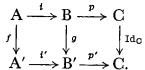
\includegraphics[keepaspectratio]{images/part002_08e8b4be.jpg}}

\begin{enumerate}
\def\labelenumi{(\roman{enumi})}
\setcounter{enumi}{3}
\tightlist
\item
  若 \(b \in \mathbf{B}\) 且 \(a' \in \mathbf{A}'\)，则
\end{enumerate}

\[
g (b) i ^ {\prime} \left(a ^ {\prime}\right) g (b) ^ {- 1} = i ^ {\prime} (\omega (b) a ^ {\prime}).
\]

\begin{enumerate}
\def\labelenumi{(\roman{enumi})}
\tightlist
\item
  对于 A 中的 \(a_{1}\)、\(a_{2}\)，在 B'' 中有
\end{enumerate}

\[
\begin{array}{r l} (f (a _ {1} ^ {- 1}), i (a _ {1})) (f (a _ {2} ^ {- 1}), i (a _ {2})) & = (f (a _ {1} ^ {- 1}) (\omega (a _ {1}) f (a _ {2} ^ {- 1})), i (a _ {1}) i (a _ {2})) \\ & = (f (a _ {1} ^ {- 1}) f (a _ {1} a _ {2} ^ {- 1} a _ {1} ^ {- 1}), i (a _ {1} a _ {2})) \\ & = (f ((a _ {1} a _ {2}) ^ {- 1}, i (a _ {1} a _ {2})) \end{array}
\]

因而 \(a \mapsto (f(a^{-1}), i(a))\)\(h\) 是从 \(A\) 到 \(B''\) 的同态 h。令 \(a \in A\)、\(a' \in A'\)、\(b \in B\)；则在 \(B''\) 中，

\[
\begin{array}{r l} b h (a) b ^ {- 1} & = b f (a ^ {- 1}) a b ^ {- 1} = (\omega (b) f (a ^ {- 1})) (b a b ^ {- 1}) \\ & = f (b a ^ {- 1} b ^ {- 1}) (b a b ^ {- 1}) = h (b a b ^ {- 1}) \\ a ^ {\prime} h (a) a ^ {\prime - 1} & = a ^ {\prime} f (a ^ {- 1}) a a ^ {\prime - 1} = a ^ {\prime} f (a ^ {- 1}) (\omega (a) a ^ {\prime - 1}) a \\ & = a ^ {\prime} f (a ^ {- 1}) f (a) a ^ {\prime - 1} f (a ^ {- 1}) a = h (a) \end{array}
\]

因而 \(h(A) = D\)\(B''\) 是 B'' 的正规子群。

\begin{enumerate}
\def\labelenumi{(\roman{enumi})}
\setcounter{enumi}{1}
\tightlist
\item
  对于 \(a \in A\)，
\end{enumerate}

\[
(p \circ q) (h (a)) = p (q (f (a ^ {- 1}) a)) = p (a) = e
\]

因而 \(p \circ q\) 在 D 上是平凡的。

\begin{enumerate}
\def\labelenumi{(\roman{enumi})}
\setcounter{enumi}{2}
\tightlist
\item
  设 \(a' \in A'\) 满足 \(i'(a') = e\)；则 \(a' \in D\)，因而存在 \(a \in A\) 使得 \(a' = f(a^{-1})a\)；这蕴含 \(a = e\)，从而 \(a' = e\)；故 \(i'\) 是单射。由于 \(p\) 和 \(q\) 是满射，\(p'\) 是满射。
\end{enumerate}

令 \(r\) 表示从 \(B''\) 到 \(B'\) 的典范态射。设 \(a' \in A'\)、\(b \in B\)，且 \(b' = r(a'b)\)。若 \(b' \in \operatorname{Im}(i')\)，则存在 \(a_1' \in A'\) 使得 \(b' = r(a_1')\)；于是存在 \(a \in A\) 使得 \(a'b = a_1'f(a^{-1})a\)，从而 \(b = a \in A\)，且

\[
p ^ {\prime} (b ^ {\prime}) = p (q (a ^ {\prime} b)) = p (b) = e;
\]

因此，\(\operatorname{Im}(i') \subset \operatorname{Ker}(p')\)。仍用 \(a', b, b'\) 表示上述对象，但假设 \(b' \in \operatorname{Ker}(p')\)；于是 \(e = p'(b') = p(q(a'b)) = p(b)\)，从而 \(b \in A\)，故

\[
b ^ {\prime} = r (a ^ {\prime} f (b) f (b ^ {- 1}) b) = r (a ^ {\prime} f (b)) \in \operatorname{Im} (i ^ {\prime});
\]

因此 \(\operatorname{Ker}(p') \subset \operatorname{Im}(i')\)。

若 \(a\in \mathbf{A}\)，则

\[
i ^ {\prime} (f (a)) = r (f (a)) = r (f (a) f \left(a ^ {- 1}\right) a) = r (a) = g (i (a)).
\]

若 \(b\in \mathbf{B}\)，则

\[
p ^ {\prime} (g (b)) = p (b)
\]

从而图 (4) 交换。

\begin{enumerate}
\def\labelenumi{(\roman{enumi})}
\setcounter{enumi}{3}
\tightlist
\item
  设 \(b \in \mathbf{B}\)、\(a' \in \mathbf{A}'\)。则
\end{enumerate}

\[
\begin{array}{r} g (b) i ^ {\prime} (a ^ {\prime}) g (b) ^ {- 1} = r (b) r (a ^ {\prime}) r (b) ^ {- 1} = r (b a ^ {\prime} b ^ {- 1}) \\ = r (\omega (b) a ^ {\prime}) = i ^ {\prime} (\omega (b) a ^ {\prime}). \end{array}
\]

命题 20. 设 G 是有限维实李群。

\begin{enumerate}
\def\labelenumi{(\roman{enumi})}
\item
  存在一个复李群 \(\tilde{\mathbf{G}}\) 和一个从 \(\mathbf{R}\) 到 \(\gamma\) 的 \(\mathbf{G}\)-解析态射 \(\tilde{\mathbf{G}}\)，具有如下性质：对于每个复李群 \(\mathbf{H}\) 以及每个从 \(\mathbf{R}\) 到 \(\phi\) 的 \(\mathbf{G}\)-解析态射 \(\mathbf{H}\)，存在唯一一个从 \(\mathbf{C}\) 到 \(\psi\) 的 \(\tilde{\mathbf{G}}\)-解析态射 \(\mathbf{H}\)，使得 \(\phi = \psi \circ \gamma\)。
\item
  若 \((\tilde{\mathbf{G}}', \gamma')\) 与 \((\tilde{\mathbf{G}}, \gamma)\) 具有相同性质，则存在唯一一个从 \(\theta\) 到 \(\tilde{\mathbf{G}}\) 的同构 \(\tilde{\mathbf{G}}'\)，使得 \(\theta \circ \gamma = \gamma'\)。
\item
  延拓 \(\mathbf{C}\) 的从 \(\mathrm{L}(\mathrm{G}) \otimes \mathbf{C}\) 到 \(\mathrm{L}(\tilde{\mathrm{G}})\) 的 \(\mathrm{L}(\gamma)\)-线性映射是满射；特别地，\(\dim_{\mathbf{C}}(\tilde{\mathbf{G}}) \leqslant \dim_{\mathbf{R}}(\mathrm{G})\)。
\end{enumerate}

断言 (ii) 是显然的。我们证明具有性质 (i) 和 (iii) 的有序对 \((\tilde{G},\gamma)\) 的存在性。

\begin{enumerate}
\def\labelenumi{(\alph{enumi})}
\tightlist
\item
  首先假设 \(G\) 连通。令 \(g = L(G)\)，\(g_{\mathbf{C}} = g \otimes_{\mathbf{R}} \mathbf{C}\) 为 \(g\) 的复化，令 \(S\)（分别地，\(S'\)）为李代数为 \(g\)（分别地，\(g_{\mathbf{C}}\)）的单连通实（分别地，复）李群，并令 \(\sigma\) 为唯一的从 \(\mathbf{R}\) 到 \(S\) 的 \(S'\)-解析态射，使得 \(L(\sigma)\) 是从 \(g\) 到 \(g_{\mathbf{C}}\) 的典范嵌入。令 \(\pi\) 为唯一的从 \(\mathbf{R}\) 到 \(S\) 的 \(G\)-解析态射，使得 \(L(\pi) = I d_{L(G)}\) 且 \(F = K e r \pi\)。
\end{enumerate}

\pandocbounded{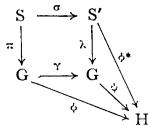
\includegraphics[keepaspectratio]{images/part002_6429af2f.jpg}}

对于每个复李群 H 以及每个从 G 到 H 的 R-解析态射 \(\phi\)，\(L(\phi): g \to L(H)\) 都有唯一的 C-线性延拓到 \(g_{C}\)，且此延拓形如 \(L(\phi^{*})\)，其中 \(\phi^{*}\) 是从 \(S'\) 到 H 的 C-解析态射。于是

\[
\mathrm{L} (\phi \circ \pi) = \mathrm{L} (\phi) \circ \mathrm{L} (\pi) = \mathrm{L} (\phi) = \mathrm{L} (\phi^ {*}) \circ \mathrm{L} (\sigma) = \mathrm{L} (\phi^ {*} \circ \sigma)
\]

因而 \(\phi \circ \pi = \phi^{*} \circ \sigma\)。所以 \(\phi^{*}(\sigma(F)) = \phi(\pi(F)) = \{e\}\)，从而

\[
\sigma (\mathrm{F}) \subset \operatorname{Ker} \phi^ {*}.
\]

令 P 为所有 \(\phi^{*}\) 变化时的 Ker \(\phi\) 的交。这是 \(S'\) 的正规李子群（第 2 号，命题 1 的推论 3）。令 \(\tilde{G} = S'/P\)，令 \(\lambda: \mathbf{S}' \to \tilde{\mathbf{G}}\) 为典范态射。于是 \(\sigma(\mathbf{F}) \subset \mathbf{P}\)，因而存在唯一一个从 \(\mathbf{R}\) 到 \(\gamma\) 的 \(\mathbf{G}\)-解析态射 \(\tilde{\mathbf{G}}\)，使得 \(\gamma \circ \pi = \lambda \circ \sigma\)。若 \(\psi: \tilde{\mathbf{G}} \to \mathbf{H}\) 表示由 \(\phi^*\) 在取商时导出的态射，则

\[
(\phi \circ \gamma) \circ \pi = \psi \circ (\lambda \circ \sigma) = \phi^ {*} \circ \sigma = \phi \circ \pi
\]

从而 \(\psi \circ \gamma = \phi\)。显然，\(\mathrm{L}(\psi)\)，进而 \(\psi\)，由等式 \(\psi \circ \gamma = \phi\) 唯一确定。因此我们证明了有序对 \((\tilde{G}, \gamma)\) 具有性质 (i) 和 (iii)。

\begin{enumerate}
\def\labelenumi{(\alph{enumi})}
\setcounter{enumi}{1}
\tightlist
\item
  现在转到一般情形。令 \(\mathbf{F}\) 为 \(\mathrm{G},\mathrm{M} = \mathrm{G} / \mathrm{F}\) 的单位分支，，令 \(i\colon \mathrm{F}\to \mathrm{G}\) 和 \(p\colon \mathrm{G}\rightarrow \mathrm{M}\) 为典范态射。我们将证明的部分 (a) 应用于 F。得到有序对 \((\tilde{\mathbf{F}},\delta)\)。对于所有 \(g\in \mathrm{G}\)，内自同构 Int \(g|\mathrm{F} = \omega '(g)\) 是 F 的自同构。由 \(\tilde{\mathbf{F}}\) 的泛性质，存在唯一一个复李群 \(\omega (g)\) 的自同构 \(\tilde{\mathbf{F}}\)，使得 \(\delta \circ \omega '(g) = \omega (g)\circ \delta\)。显然，\(\omega\) 是从 G 到 \(\operatorname {Aut}(\tilde{\mathbf{F}})\) 的态射。若 \(g\in \mathbf{G}\) 且 \(f\in \tilde{\mathbf{F}}\)，则
\end{enumerate}

\[
\delta (g f g ^ {- 1}) = (\delta \circ \omega^ {\prime} (g)) (f) = (\omega (g) \circ \delta) (f) = \omega (g) (\delta (f)).
\]

若 \(f \in \mathbf{F}\)，则 \(\delta \circ (\operatorname{Int}_{\mathbb{F}} f) = (\operatorname{Int}_{\tilde{\mathbb{F}}} \delta(f)) \circ \delta\)，且 \(\operatorname{Int}_{\tilde{\mathbb{F}}} \delta(f)\) 是复李群 \(\tilde{\mathbf{F}}\) 的自同构；故 \(\operatorname{Int}_{\tilde{\mathbb{F}}} \delta(f) = \omega(f)\)。

因此可应用引理 7，从而得到交换图

\[
\begin{array}{c} \mathrm{F} \xrightarrow {i} \mathrm{G} \xrightarrow {p} \mathrm{M} \\ \delta \Big \downarrow \qquad \qquad \qquad \gamma \Big \downarrow \qquad \qquad \Big \downarrow \mathrm{Id} \\ \tilde {\mathrm{F}} \xrightarrow {\tilde {i}} \tilde {\mathrm{G}} \xrightarrow {\tilde {p}} \mathrm{M}. \end{array}
\]

借助 \(\tilde{\mathbf{F}}\)，将 \(\tilde{\mathbf{G}}\) 识别为 \(\tilde{i}\) 的正规子群。群 \(\tilde{\mathbf{G}}\) 由 \(\tilde{\mathbf{F}}\) 和 \(\gamma (\mathbf{G})\) 生成；因此，由 \(\tilde{\mathbf{F}}\) 的元素定义的 \(\tilde{\mathbf{G}}\) 的自同构都是复李群结构的自同构。由 § 1，第 9 号，命题 18，\(\tilde{\mathbf{G}}\) 上存在唯一一个复李群结构，使得 \(\tilde{\mathbf{F}}\) 是 \(\tilde{\mathbf{G}}\) 的开李子群。以下 \(\tilde{\mathbf{G}}\) 均取此结构。由于 \(\delta\) 是 \(\mathbf{R}\)-解析的，\(\gamma\) 也是 \(\mathbf{R}\)-解析的。

有序对 \((\tilde{G},\gamma)\) 具有命题的性质 (iii)。我们证明它具有性质 (i)。设 H 是复李群，\(\phi\) 是从 G 到 H 的 R-解析态射。存在一个从 \(\eta\) 到 H 的 C-解析态射 \(\tilde{F}\)，使得 \(\eta \circ \delta = \phi |F\)。设 \(g\in G\)。映射

\[
f \mapsto \eta (\omega (g) f), \quad f \mapsto \phi (g) \eta (f) \phi (g) ^ {- 1}
\]

从 \(\tilde{\mathbf{F}}\) 到 \(\mathbf{H}\) 都是 \(\mathbf{C}\)-解析态射；它们在 \(\delta(\mathbf{F})\) 上一致，因为若 \(f' \in \mathbf{F}\)，则

\[
\begin{array}{r} \phi (g) \eta (\delta (f ^ {\prime})) \phi (g) ^ {- 1} = \phi (g) \phi (f ^ {\prime}) \phi (g) ^ {- 1} = \phi (g f ^ {\prime} g ^ {- 1}) \\ = \eta (\delta (g f ^ {\prime} g ^ {- 1})) = \eta (\omega (g) \delta (f ^ {\prime})); \end{array}
\]

因此对于所有 \(\eta (\omega (g)f) = \phi (g)\eta (f)\phi (g)^{-1}\) 和所有 \(g\in G\)，都有 \(f\in \tilde{\mathbf{F}}\)。若 \(\mathbf{G}'\) 表示关于 \(\mathbf{G}\) 的 \(\tilde{\mathbf{F}}\) 与 \(\omega\) 的半直积，则存在从群 \(\zeta\) 到 \(\mathbf{G}'\) 的态射 \(\mathrm{H}\)，它在 \(\phi\) 上与 \(\mathrm{G}\) 一致，在 \(\eta\) 上与 \(\tilde{\mathbf{F}}\) 一致。对于 \(f\in \mathbf{F}\)，

\[
\zeta (\delta (f ^ {- 1}) f) = \eta (\delta (f ^ {- 1})) \phi (f) = \phi (f ^ {- 1}) \phi (f) = e.
\]

因此 \(\zeta\) 在取商后定义出从 \(\psi\) 到 H 的态射 \(\tilde{\mathbf{G}}\)。于是 \(\psi \circ \gamma = \phi\) 且 \(\psi \circ \tilde{i} = \eta\)；后一个等式蕴含 \(\psi\) 是 C-解析的。

最后，设 \(\psi'\) 是从 \(\mathbf{C}\) 到 \(\tilde{\mathbf{G}}\) 的 \(\mathbf{H}\)-解析态射，满足 \(\phi = \psi' \circ \gamma\)。则

\[
\psi^ {\prime} \circ \tilde {i} \circ \delta = \psi^ {\prime} \circ \gamma \circ i = \phi \circ i = \psi \circ \tilde {i} \circ \delta
\]

因而 \(\psi' \circ \tilde{i} = \psi \circ \tilde{i}\)。由于 \(\tilde{G}\) 由 \(\tilde{i}(\tilde{\mathrm{F}})\) 和 \(\gamma(G)\) 生成，\(\psi' = \psi\)。

定义 4. \((\tilde{G},\gamma)\)，或简记为 \(\tilde{G}\)，称为 G 的泛复化。

注记。(1) 设 \((\tilde{\mathbf{G}},\gamma)\) 是 G 的泛复化。设 \(G_0\)（分别地，\(\tilde{G}_0\)）为 G（分别地，\(\tilde{G}\)）的单位分支。由命题 20 的证明，\((\tilde{G}_0,\gamma |G_0)\) 是 \(G_0\) 的泛复化，且复合态射

\[
\mathrm{G} \rightarrow \tilde {\mathrm{G}} \rightarrow \tilde {\mathrm{G}} / \tilde {\mathrm{G}} _ {0}
\]

在取商后定义出从 \(\mathbf{G} / \mathbf{G}_0\) 到 \(\tilde{\mathbf{G}} / \tilde{\mathbf{G}}_0\) 的同构。

\begin{enumerate}
\def\labelenumi{(\arabic{enumi})}
\setcounter{enumi}{1}
\tightlist
\item
  假设 G 单连通。令 \(g = L(G)\)，令 \(g_{c}\) 为 g 的复化，令 \(S'\) 为李代数为 \(g_{c}\) 的单连通复李群，令 \(\sigma\) 为从 G 到 \(S'\) 的态射，使得 \(L(\sigma)\) 是从 g 到 \(g_{c}\) 的典范嵌入。我们再次使用命题 20 的证明中部分 (a) 的记号。若 \(H = S'\) 且 \(\phi = \sigma\)，则 \(\phi^{*} = I d_{g}\)。因此 \((S', \sigma)\) 是 G 的泛复化。注意 \(\sigma\) 一般并非单射（练习 16）；然而由于 \(L(\sigma)\) 是单射，其核是离散的。另一方面，令 \(\theta\) 为由 g 定义的 \(g_{c}\) 的对合，令 \(\eta\)\(S'\) 为 S' 的底层实李群所对应的自同构；令 \(S'^{\eta}\)\(S'\) 为 S' 中在 \(\eta\)\(S'\) 下不变的点的集合；它是 S' 的实李子群，其李代数为 g（§3，第 8 号，命题 29 的推论 1）。由第 1 号、命题 1 的推论 1，\(\sigma(G)\)\(S'\) 是 S' 的李代数为 g 的实积分子群，因而 \(\sigma(G)\) 是 \(S'^{\eta}\) 的单位分支；特别地，\(\sigma(G)\)\(S'\) 是 S' 的实李子群。
\end{enumerate}

\section{超度量域上的李群}

本节假定赋值域 K 是超度量的且特征为 0。令 A 表示 K 的赋值环，m 表示 A 的极大理想，p 表示剩余域 A/m 的特征。若 K 是局部紧的，则 \(p \neq 0\)（交换代数，第 VI 章，§ 9，定理 1）。

\subsection{从李代数到李群}

命题 1. 设 G 是单位元为 e 的李群芽。G 中存在一个由 G 的李子群组成的 e 的开邻域基。

给 \(\mathrm{L}(\mathrm{G})\) 赋予一个与其拓扑相容的范数，并使得对 \(\| [x,y]\| \leqslant \| x\| \| y\|\) 中所有 \(x,y\) 都有 \(\mathrm{L}(\mathrm{G})\)。令 \(\mathrm{G}_1\) 为由 \(\mathrm{L}(\mathrm{G})\) 定义的李群。由 § 4，第 2 号，定理 2，G 与 \(\mathrm{G}_1\) 局部同构。因此只需应用 § 4，第 2 号，引理 3 (iii)。

定理 1. 设 \(\mathbf{L}\) 是完备可赋范李代数。存在一个李群 \(\mathbf{G}\)，使得 \(\mathbf{L}(\mathbf{G})\) 同构于 \(\mathbf{L}\)。任意两个这样的群都局部同构。

第一个断言已在 § 4，第 2 号，引理 3 中证明。第二个断言是 § 4，第 2 号，定理 2 的特例。

定理 2. 设 G 是李群，b 是 L(G) 的具有拓扑补空间的李子代数。存在 G 的李子群 H，使得 L(H) = b。若 H₁ 和 H₂ 是 G 的李子群，且 L(H₁) = L(H₂) = b，则 H₁ ∩ H₂ 在 H₁ 和 H₂ 中都是开集。

第一个断言由命题 1 和 §4，第 2 号，定理 3 得到。第二个断言是 §4，第 2 号，定理 3 的特例。

定理 3. 设 \(\mathbf{G}\) 和 \(\mathbf{H}\) 是李群，\(h\) 是从 \(\mathbf{L}(\mathbf{G})\) 到 \(\mathbf{L}(\mathbf{H})\) 的连续态射。

\begin{enumerate}
\def\labelenumi{(\roman{enumi})}
\item
  存在 \(\mathbf{G}'\) 的开子群 \(\mathbf{G}\) 以及从 \(\phi\) 到 \(\mathbf{G}'\) 的李群态射 \(\mathbf{H}\)，使得 \(h = \mathbf{L}(\phi)\)。
\item
  设 \(\mathbf{G}_1, \mathbf{G}_2\) 是 \(\mathbf{G}\) 的开子群，\(\phi_i\) 是从 \(\mathbf{G}_i\) 到 \(\mathbf{H}\) 的态射，且 \(h = \mathbf{L}(\phi_i)\)。则 \(\phi_1\) 与 \(\phi_2\) 在 \(\mathbf{G}\) 的某个开子群上相同。
\end{enumerate}

由命题 1，这由 § 4，第 1 号，定理 1 得到。

命题 2. 设 \(\mathbf{G}\) 是李群，\(\mathfrak{h}\) 是 \(\mathbf{L}(\mathbf{G})\) 的具有拓扑补空间的李子代数。下列条件等价：

\begin{enumerate}
\def\labelenumi{(\roman{enumi})}
\item
  存在 \(\mathbf{G}'\) 的开子群 \(\mathbf{G}\) 以及 \(\mathbf{H}\) 的正规李子群 \(\mathbf{G}'\)，使得 \(\mathrm{L(H)} = \mathfrak{h}\)。
\item
  \(\mathfrak{h}\) 是 \(\mathrm{L}(\mathrm{G})\) 的理想。
\end{enumerate}

若存在具有 (i) 中性质的 \(G'\)\(H\) 和 H，则由 § 3，第 12 号，命题 47，有 \(L(G') = L(G)\)，且 \(L(H)\) 是 \(L(G')\) 的理想。

假设 \(\mathfrak{h}\) 是 \(\mathrm{L}(\mathrm{G})\) 的理想。存在一个李群 \(\mathrm{F}\)，使得 \(\mathrm{L}(\mathrm{F}) = \mathrm{L}(\mathrm{G}) / \mathfrak{h}\)（定理 1）。令 h 为从 \(h\)\(\mathrm{L}(\mathrm{G})\) 到 \(\mathrm{L}(\mathrm{F})\) 的典范态射。由定理 3 (i)，存在 \(\mathrm{G}'\) 的开子群 \(\mathrm{G}\) 以及从 \(\phi\) 到 \(\mathrm{G}'\) 的李群态射 \(\mathrm{F}\)，使得 \(\mathrm{L}(\phi) = \mathrm{h}\)。由 § 3，第 8 号，\(\mathrm{H}\) 的核 \(\phi\) 是 \(\mathrm{G}'\) 的李子群，且 \(\mathrm{L}(\mathrm{H}) = \mathrm{Ker} \, \mathrm{L}(\phi) = \mathrm{Ker} \, h = \mathfrak{h}\)。最后，由于 ，\(\mathrm{H}\) 是 \(\mathrm{G}'\)\(\mathrm{H} = \mathrm{Ker} \, \phi\) 的正规子群。

\subsection{指数映射}

命题 3. 设 \(\mathbf{G}\) 是李群。存在 \(\phi\) 的指数映射 \(\mathbf{G}\)，具有如下性质：

\begin{enumerate}
\def\labelenumi{(\roman{enumi})}
\item
  \(\phi\) 定义在加法群 L(G) 的开子群 U 上；
\item
  \(\phi (\mathbf{U})\) 是 \(\mathbf{G}\) 的开子群，且 \(\phi\) 是从解析流形 \(\mathbf{U}\) 到解析流形 \(\phi (\mathbf{U})\) 的同构；
\item
  对所有 \(\phi(nx) = \phi(x)^n\) 和所有 \(x \in \mathbf{U}\)，都有 \(n \in \mathbf{Z}\)。
\end{enumerate}

给 \(\dot{\mathrm{L}}(\mathrm{G})\) 赋予一个与其拓扑相容的范数，并使得对 \(\| [x,y]\| \leqslant \| x\| \| y\|\) 中的 \(x,y\) 有 \(\mathrm{L}(\mathrm{G})\)。令 \(\mathbf{G}_1\) 为由 \(\mathrm{L}(\mathrm{G})\) 定义的李群。令 \(\psi = \mathrm{Id}_{\mathrm{G}_1}\)，它是 \(\mathbf{G}_1\) 的一个指数映射。对所有 \(\mu >0\)，令 \(\mathrm{L}_{\mu}\) 为满足 \(x\in \mathrm{L}(\mathrm{G})\) 的 \(\| x\| < \mu\) 的集合。于是，当 \(\mu\) 充分小时，\(\mathrm{L}_{\mu}\) 是加法群 \(\mathrm{L}(\mathrm{G}),\psi (\mathrm{L}_{\mu})\)\(\mathrm{G}_1\) 的开子群，\(\psi |\mathrm{L}_{\mu}\) 是 \(\mathrm{L}_{\mu}\) 的开子群（§ 4，第 2 号，引理 3），\(\psi (\mathrm{L}_{\mu})\) 是从解析流形 \(\psi (nx) = \psi (x)^n\) 到 \(x\in \mathrm{L}_{\mu}\) 的解析流形同构，并且对所有 \(n\in \mathbf{Z}\) 和所有 \(\mathrm{L}_{\mu}\)，有 \(\mathrm{L}(\mathrm{G})\)。\(\mu\) 构成  中 0 的邻域基。由定理 1，存在 \(\mathbf{G}'\) 以及 \(\mathbf{G}\) 的开子群 \(\psi (\mathrm{L}_{\mu})\)，使得  与 \(\mathbf{G}'\) 同构，从而得到命题。

命题 4. 设 G 是李群，\(\phi\) 是 G 的单射指数映射。假设 \(p > 0\)。对 L(G) 中所有 \(x, y\)，

\begin{enumerate}
\def\labelenumi{(\arabic{enumi})}
\tightlist
\item
\end{enumerate}

\[
x + y = \lim _ {n \rightarrow + \infty} p ^ {- n} \phi^ {- 1} (\phi (p ^ {n} x) \phi (p ^ {n} y))\tag{1}
\]

\[
[ x, y ] = \lim _ {n \rightarrow + \infty} p ^ {- 2 n} \phi^ {- 1} (\phi (p ^ {n} x) \phi (p ^ {n} y) \phi (- p ^ {n} x) \phi (- p ^ {n} y)).\tag{2}
\]

这些是 § 4，第 3 号，命题 4 的特例。

\subsection{标准群†}

若 \(\mathrm{S}(\mathbf{X}_{1},\mathbf{X}_{2},\ldots,\mathbf{X}_{n})\) 是系数在 A 中的形式幂级数，则对于 m 中的所有 \(x_{1},\ldots,x_{r}\)，级数 \(\mathrm{S}(x_{1},x_{2},\ldots,x_{r})\) 收敛。更确切地说，\(m\times m\times\cdots\times m\) 包含于 S 的绝对收敛域（可微与解析流形，R，4.1.3）。

定义 1. 设 \(r\) 是满足 \(\geqslant 0\)\(r\)\(\mathbf{K}\)\(G\) 的整数。K 上 r 维的标准群是具有下列性质的李群 G：

\begin{enumerate}
\def\labelenumi{(\roman{enumi})}
\item
  G 的底层解析流形是 m × m × · · · × m（r 个因子）；
\item
  存在一个以 \(\mathbf{F}\) 为系数、无常数项的关于 \(2r\) 个变量的形式幂级数 \(\mathbf{A}^r\)，使得对 G 中所有 \(x.y = \mathbf{F}(x,y)\)，都有 \(x,y\)\(\mathbf{G}\)。
\end{enumerate}

于是 0.0 = 0，从而 G 的单位元是 m × m · · · × m 的原点。
† 第 3、4 号的结果及其证明在 K 的特征为正时仍然成立。

将 L(G) 识别为 \(K^r\)。由 § 5，公式 (13)，L(G) 关于典范基的结构常数属于 A。在同一证明中，我们需要把 m × ⋯ × m 中的元素既看作 G 的元素，又看作 L(G) 的元素。

例。设 \(G = 1 + \mathbf{M}_{n}(m)\)，它是 \(\mathbf{M}_{n}(\mathbf{K})\) 的开子集。若 \(x \in G\)，则 det \(x \in 1 + m\)，因而 \(G \subset \mathbf{GL}(n, K)\)。显然 \(GG \subset G\)。若 \(x = 1 + y\)，其中 \(y \in \mathbf{M}_{n}(m)\)，则矩阵求逆的计算首先说明 \(x^{-1} \in \mathbf{M}_{n}(\mathbf{A})\)；若写作 \(x^{-1} = 1 + y'\)，则 \(y + y' + yy' = 0\)，从而 \(y' \in \mathbf{M}_{n}(m)\)，因此 \(x^{-1} \in G\)。所以 G 是 \(\mathbf{GL}(n, K)\) 的开子群。我们借助映射 \(m^{n^2}\) 将 G 与 \((\delta_{ij} + y_{ij}) \mapsto (y_{ij})\) 识别。显然 G 是标准群。

定理 4. 设 G 是有限维李群。G 存在一个开子群同构于标准群。

将 G 替换为与 G 的某个开子群同构的群后，问题归结为 G 是 \(K^{r}\) 的开子集，单位元为 0，且乘积 x.y 和逆元 \(x^{[-1]}\) 的坐标由下列公式给出：

\begin{enumerate}
\def\labelenumi{(\arabic{enumi})}
\setcounter{enumi}{2}
\tightlist
\item
\end{enumerate}

\[
(x. y) _ {i} = x _ {i} + y _ {i} + \sum_ {| \alpha | \geqslant 1, | \beta | \geqslant 1} c _ {\alpha \beta i} x ^ {\alpha} y ^ {\beta} (i = 1, 2, \dots , r)\tag{3}
\]

\[
(x ^ {[ - 1 ]}) _ {i} = - x _ {i} + \sum_ {| \alpha | > 1} d _ {\alpha i} x ^ {\alpha} \quad (i = 1, 2, \dots , r)\tag{4}
\]

令 \(x, y\)\(G\)\(\lambda \in K^*\)\(G\)，通过比为 \(G' = \lambda G\) 的位似将群运算从 G 搬到 \(\lambda\)。对于 G' 中的 \(x', y'\)\(G'\)，在 G' 中计算的乘积 \(x'.y'\) 和逆元 \(x'^{(-1)}\)\(G'\) 的坐标为

\[
(x ^ {\prime}. y ^ {\prime}) _ {i} = x _ {i} ^ {\prime} + y _ {i} ^ {\prime} + \sum_ {| \alpha | \geqslant 1, | \beta | \geqslant 1} c _ {\alpha \beta i} ^ {\prime} x ^ {\prime \alpha} y ^ {\prime \beta} (i = 1, 2, \dots , r)
\]

\[
(x ^ {\prime [ - 1 ]}) _ {i} = - x _ {i} ^ {\prime} + \sum_ {| \alpha | > 1} d _ {\alpha i} ^ {\prime} x ^ {\prime \alpha} \quad (i = 1, 2, \dots , r)
\]

其中

\[
c _ {\alpha \beta i} ^ {\prime} = \lambda^ {- | \alpha | - | \beta | + 1} c _ {\alpha \beta i}, \quad d _ {\alpha i} ^ {\prime} = \lambda^ {- | \alpha | + 1} d _ {\alpha i}.
\]

由于级数 (3) 和 (4) 收敛可知，当 \(|\lambda|\) 充分大时，对所有 \(\alpha, \beta, i\)，

\[
\left| c _ {\alpha \beta i} ^ {\prime} \right| \leqslant 1, \quad \left| d _ {\alpha i} ^ {\prime} \right| \leqslant 1
\]

即 \(c_{\alpha\beta i}^{\prime}\in A\) 且 \(d_{\alpha i}^{\prime}\in A\)；另一方面 \(G^{\prime}\supset m\times m\times\cdots\times m\)。于是 \(m\times m\times\cdots\times m\) 是 \(G^{\prime}\) 的开子群，且是标准群。

\subsection{标准群的滤过}

我们再次采用定义 1 的记号。选取一个数 \(a > 1\) 和 K 的实赋值 \(v\)\(\mathbf{K}\)，使得对所有 \(|x| = a^{-v(x)}\) 都有 \(x \in \mathbf{K}\)\(a\)（交换代数，第 VI 章，§6，命题 3）。若 a 是 A 的包含于 m 中的非零（因而是开的）理想，令 \(\mathrm{G}(a)\)\(a\) 表示坐标属于 a 的 G 中元素的集合。若 \(\lambda \in \mathbf{R}\)，令 \(a_{\lambda}\)（分别地，\(a_{\lambda}^{+}\)）表示满足 \(x \in \mathbf{K}\)（分别地，\(v(x) \geqslant \lambda\)）的 \(v(x) > \lambda\) 的集合；于是 \(a_0 = A\)，\(a_0^+ = m\)。对于 \(x = (x_1, \ldots, x_r) \in G\)，记

\[
\omega (x) = \inf (v (x _ {1}), \dots , v (x _ {r})).\tag{5}
\]

命题 5. 设 G 是标准群。

\begin{enumerate}
\def\labelenumi{(\roman{enumi})}
\item
  若 \(\mathfrak{a}\) 是包含于 \(\mathbf{A}\) 中的 \(\mathfrak{m}\) 的非零理想，则 \(\mathbf{G}(\mathfrak{a})\) 是 \(\mathbf{G}\) 的开正规子群。
\item
  当 \(\mathbf{G}(\mathfrak{a}_{\lambda})\) 时，\(\lambda > 0\)\(e\) 构成 \(\mathbf{G}\) 中 e 的邻域基。
\item
  假设 \(\mathfrak{a}_{\lambda} \subset \mathfrak{a}\)（当 \(\lambda \geqslant \lambda_0\) 时），并给 \(G(\mathfrak{a}) / G(\mathfrak{a}_{\lambda})\) 赋予离散拓扑（当 \(\lambda \geqslant \lambda_0\) 时）。则拓扑群 \(G(\mathfrak{a})\) 是各群 \(G(\mathfrak{a}) / G(\mathfrak{a}_{\lambda})\) 的逆极限。
\item
  设 \(\mathfrak{a},\mathfrak{b}\) 是包含于 \(\mathfrak{m}\) 中的 A 的非零理想，满足 \(\mathfrak{a} \supset \mathfrak{b} \supset \mathfrak{a}^2\)。从 G(a) 到 (a/b) × · · · × (a/b) 的映射 \(x \mapsto (x_1 \bmod \mathfrak{b}, \ldots, x_r \bmod \mathfrak{b})\) 在取商后定义出从 G(a)/G(b) 到加法群 (a/b) × · · · × (a/b) 的同构。
\end{enumerate}

若 \(x \in G\) 且 \(y \in G(a)\)\(x\)\(x.y\)\(a\)，则 x 和 x.y 的坐标模 a 相等。因此，对于 G 中的 \(x'\)、\(x''\)\(G\) 以及 G(a) 中的 \(y'\)、\(y''\)\(G(a)\)\(x'.x''\)\((x'.y')\)\((x''.y'')\)\(a\)，x'.x'' 与 (x'.y') . (x''.y'') 的坐标模 a 相等。这证明了 (i)。

\begin{enumerate}
\def\labelenumi{(\roman{enumi})}
\setcounter{enumi}{1}
\item
  显然。
\item
  由上可知，这由一般拓扑，第 III 章，§ 7，命题 2 得到。
\end{enumerate}

若 \(x \in G(a)\) 且 \(y \in G(a)\)\(x, y\)\(x + y\)，则由 § 5 的公式 (4)，x、y 的坐标与 x + y 的坐标模 \(G(a^2)\) 同余。这证明了 (iv)。

推论。假设 K 局部紧，令 \(q = \operatorname{Card}(\mathbf{A} / \mathfrak{m})\)。

\begin{enumerate}
\def\labelenumi{(\roman{enumi})}
\item
  若 \(a = m^{a}\) 且 \(b = m^{b}\)，其中 \(b \geqslant a \geqslant 1\)，则 \(\mathrm{G}(a)/\mathrm{G}(b)\) 是基数为 \(q^{r(b-a)}\) 的 p-群。
\item
  G(a) 是 p-群的逆极限。
\end{enumerate}

\(\mathrm{G}(\mathfrak{a})/\mathrm{G}(\mathfrak{b})\) 中元素的数目是 \((\mathrm{Card}(\mathfrak{a}/\mathfrak{b}))^{r}\)；若 \(b=a+1\)，则 a/b 是 A/m 上的一维向量空间，从而在此情形下得到 (i)；一般情形由对 b-a 作归纳得到。断言 (ii) 由 (i) 和命题 5 (iii) 得到。

命题 6. 设 \(\mathfrak{a}, \mathfrak{b}, \mathfrak{c}, \mathfrak{c}'\) 是包含于 \(\mathbf{A}\) 中的 \(\mathfrak{m}\) 的非零理想，满足

\[
\mathfrak {c} ^ {\prime} \subset \mathfrak {c}, \quad \mathfrak {a b} \subset \mathfrak {c}, \quad \mathfrak {a b} ^ {2} \subset \mathfrak {c} ^ {\prime}, \quad \mathfrak {a} ^ {2} \mathfrak {b} \subset \mathfrak {c} ^ {\prime}.
\]

若 \(x \in \mathrm{G}(\mathfrak{a})\) 且 \(y \in \mathrm{G}(\mathfrak{b})\)，则 \(x^{[-1]}y^{[-1]}x.y, x.y.x^{[-1]}y^{[-1]}\)、 和 \([x,y]\) 属于 \(\mathrm{G}(\mathfrak{c})\)，并且模 \(\mathrm{G}(\mathfrak{c}')\) 同余。

由 § 5，第 2 号，命题 1，存在 \(c_{\alpha \beta} \in \mathbf{A}^r\)，使得

\[
x ^ {[ - 1 ]}. y ^ {[ - 1 ]}. x. y - [ x, y ] = \sum_ {| \alpha | + | \beta | \geqslant 3} c _ {\alpha \beta} x ^ {\alpha} y ^ {\beta}.
\]

若 \(x = 0\) 或 \(y = 0\)，则 \(x^{[-1]}y^{[-1]}x.y - [x,y] = 0\)；因此 \(c_{0\beta} = c_{\alpha 0} = 0\)。另一方面，条件

\[
x \in \mathrm{G} (\mathfrak {a}), \quad y \in \mathrm{G} (\mathfrak {b}), \quad | \alpha | \geqslant 1, \quad | \beta | \geqslant 1, \quad | \alpha | + | \beta | \geqslant 3
\]

蕴含

\[
c _ {\alpha \beta} x ^ {\alpha} y ^ {\beta} \in \mathrm{G} (a ^ {2} b + a b ^ {2}) \subset \mathrm{G} (c ^ {\prime})
\]

因而 \(x^{[-1]} \cdot y^{[-1]}x \cdot y - [x, y] \in \mathrm{G}(\mathfrak{c}')\)。类似地可得

\[
x. y. x ^ {[ - 1 ]}. y ^ {[ - 1 ]} - [ x, y ] \in \mathrm{G} (\mathfrak {c} ^ {\prime}).
\]

最后，由 § 5，公式 (13)，\([x,y] \in G(\mathfrak{ab}) \subset G(\mathfrak{c})\)。

命题 7. (i) 族 \((\mathrm{G}(\mathfrak{a}_{\lambda}))\) 是 \(\mathbf{G}\) 上的中心滤过（第二章，§ 4，第 4 号，定义 2）。

\[
\text { (ii) } For \lambda \in \mathbf {R} _ {+} ^ {*}, G (a _ {\lambda}) = \{x \in G | \omega (x) \geqslant \lambda \}, G (a _ {\lambda} ^ {+}) = \{x \in G | \omega (x) > \lambda \}.
\]

\begin{enumerate}
\def\labelenumi{(\roman{enumi})}
\setcounter{enumi}{1}
\tightlist
\item
  显然。我们证明 (i)。显然 \(G(a_{\lambda}) = \bigcap_{\mu < \lambda} G(a_{\mu})\)，且 \(G = \bigcup_{\lambda > 0} G(a_{\lambda})\)。另一方面，若 \(x \in G(a_{\lambda})\) 且 \(y \in G(a_{\mu})\)，则
\end{enumerate}

\[
x ^ {[ - 1 ]}. y ^ {[ - 1 ]}. x. y \in G (a _ {\lambda + \mu})
\]

将命题 6 应用于 \(a = a_{\lambda}, b = a_{\mu}, c = c' = a_{\lambda + \mu}\) 得到。

由第二章，§ 4，第 4 号，我们可以构造与带中心滤过 \((G(a_\lambda))\) 的群 G 相联系的群 gr(G)。对所有 \(G_\lambda = G(a_\lambda)/G(a_\lambda^+)\) 写 \(\lambda > 0\)，得到 \(gr(G) = \bigoplus_{\lambda>0} G_\lambda\)。回忆一下（同上，命题 1），G 中的换位子使我们能够在 gr(G) 上定义括号，使 gr(G) 成为李代数，具体如下：若 \(x \in G_\lambda\) 且 \(y \in G_\mu\)，取 \(\bar{x}\) 在 \(G(a_\lambda)\) 中的一个代表元 x，以及 \(\bar{y}\) 在 \(G(a_\mu)\) 中的一个代表元 y；则 \([\bar{x},\bar{y}]\) 是 \(x^{[-1]}.y^{[-1]}.x.y \in G(a_{\lambda+\mu})\) 在 \(G_{\lambda+\mu}\) 中的类。由命题 6（取 \(a = a_\lambda, b = a_\mu, c = a_{\lambda+\mu}, c' = a_{\lambda+\mu}\)），可见 \([\bar{x},\bar{y}]\) 也是 \([x,y]\) 在 \(G_{\lambda+\mu}\) 中的类。因此，当把 G 看作由 \(K^r\)\(G(a_\lambda)\) 滤过的李子代数  时，相关分次李代数（第二章，§ 4，第 3 号）等于 gr(G)。

\subsection{标准群中的幂}

保留第 4 号的记号。

命题 8. 设 \(n \in \mathbf{Z}\)\(h_n\)，h＿n 是从 G 到 G 的映射 \(x \mapsto x^n\)\(G\)\(G\)\(a\)\(A\)\(m\)。设 a 是包含于 m 中的 A 的非零理想，且 \(n \notin a\)\(h_n|G(a)\)\(G(a)\)\(G(na)\)。则 h＿n 在 G(a) 上的限制是从解析流形 G(a) 到解析流形 G(na) 的同构。

由标准群的定义，\(h_n\) 在整个 G 上等\(G\)于一个系数在 A＾r 中的整级数。由\(A^r\) § 5，公式 (4)，此级数形如

\[
h _ {n} (x) = n x + \sum_ {| \alpha | \geqslant 2} a _ {\alpha} x ^ {\alpha}.
\]

因此，对于 \(x \in G\)，

\[
\begin{array}{r l} h _ {n} (n x) & = n ^ {2} \Big (x + \sum_ {| \alpha | \geqslant 2} a _ {\alpha} n ^ {| \alpha | - 2} x ^ {\alpha} \Big) \\ & = n ^ {2} \mathrm{S} (x) \end{array}
\]

其中我们记 \(\mathrm{S}(x)=x+\sum_{|\alpha| \geq 2} a_{\alpha} n^{|\alpha|-2} x^{\alpha}\)。此级数 \(\mathrm{S}(x)\) 定义了一个从 G 到 G 的解析映射，仍记为 S。由代数，第 IV 章，§6，命题 8，存在一个系数在  中的整级数 \(S'\)，使得 \(A^r\)\(\mathrm{S}'(\mathrm{S}(\mathrm{X}))=\mathrm{S}(\mathrm{S}'(\mathrm{X}))=\mathrm{X}\)。因此 S 是从解析流形 G 到自身的同构，并且对于 A 的任意包含于 m 中的非零理想 b，都有 \(\mathrm{S}(\mathrm{G}(\mathrm{b}))\subset\mathrm{G}(\mathrm{b}),\mathrm{S}'(\mathrm{G}(\mathrm{b}))\subset\mathrm{G}(\mathrm{b})\)、，从而

\[
\mathrm{S} (\mathrm{G} (\mathfrak {b})) = \mathrm{G} (\mathfrak {b}).
\]

由于 \(h_n(y) = n^2\mathrm{S}\left(\frac{1}{n} y\right)\) 对 \(y \in n\mathrm{G}\) 成立，可见 h＿n 在 \(h_n|n\mathrm{G}(\mathfrak{b})\)\(n\mathrm{G}(\mathfrak{b})\) 上的限制是从解析流形  到解析流形 \(n^2\mathrm{G}(\mathfrak{b})\) 的同构。但是，由于 \(n \notin \mathfrak{a}\)，对所有 \(|n| > |\lambda|\) 都有 \(\lambda \in \mathfrak{a}\)，从而 \(n^{-1}\mathfrak{a} \subset \mathfrak{m}\)，因此 \(\mathfrak{a}\) 具有形式 \(n\mathfrak{b}\)，其中 \(\mathfrak{b}\) 是包含于 \(\mathrm{A}\)\(\mathfrak{m}\) 中的 A 的非零理想。

推论。若 n 在 A 中可逆，则 h＿n 是从解析流形 G 到自身的同构。对于 A 的每个包含于 \(n\)\(h_n\)\(\mathfrak{a}\) 中的非零理想 \(\mathfrak{m}\)，都有 \(h_n(\mathrm{G}(\mathfrak{a})) = \mathrm{G}(\mathfrak{a})\)。对所有 \(x \in \mathrm{G}\)，都有 \(\omega(x^n) = \omega(x)\)。

这立即由命题 8 得到。

命题 9. 假设 \(p \neq 0\)。

\begin{enumerate}
\def\labelenumi{(\roman{enumi})}
\item
  设 \(\mathfrak{a},\mathfrak{b}\) 是 \(\mathbf{A}\) 的非零理想，满足 \(\mathfrak{b} \subset \mathfrak{a} \subset \mathfrak{m}\)。在群 \(\mathrm{G}(\mathfrak{a}) / \mathrm{G}(\mathfrak{b})\)\(p\) 中，每个元素的阶都是 p 的幂。
\item
  假设 \(v(p) = 1\)。若 \(x \in G\) 满足 \(\omega(x) > \frac{1}{p - 1}\)，则
\end{enumerate}

\[
\omega (x ^ {p}) = \omega (x) + 1.
\]

由 § 5，公式 (4)，对所有 \(x \in G\)，

\[
x ^ {p} = p x + \sum_ {| \alpha | \geqslant 2} c _ {\alpha} x ^ {\alpha}
\]

即使为了证明 (i)，也可以假设 \(c_{\alpha} \in A^{r}\)\(\alpha\)\(v(p) = 1\)。于是若 \(\omega(x) \geqslant 1\)，便有 \(\omega(x^{p}) \geqslant \omega(x) + 1\)，从而当 n 趋于 \(\omega(x^{p^{n}})\) 时 \(+\infty\)\(n\) 趋于 \(+\infty\)；这证明了 (i)。由于 \(\binom{p}{i}\)\(p\) 可被 p 整除，对于

\(1 \leqslant i \leqslant p - 1\)\(c_{\alpha} \in pA^{r}\)，§ 5，第 3 号，命题 2 说明，对于

\[
2 \leqslant | \alpha | \leqslant p - 1
\]

从而

\[
\omega \left(c _ {\alpha} x ^ {\alpha}\right) > \omega (p x) = \omega (x) + 1 \quad \text { for } 2 \leqslant | \alpha | \leqslant p - 1.
\]

另一方面，若 \(|\alpha| \geqslant p\)，则 \(\omega(c_{\alpha}x^{\alpha}) \geqslant p\omega(x)\)，而当 \(p\omega(x) > \omega(x) + 1\) 时，\(\omega(x) > \frac{1}{p - 1}\)。这证明了 (ii)。

\subsection{对数映射}

引理 1. 假设 \(p \neq 0\)\(G\)\(G_1\)\(G\)。设 G 是一个李群，G＿1 是 G 的一个同构于标准群的开子群，且 \(x \in G\)。下列条件等价：

\begin{enumerate}
\def\labelenumi{(\roman{enumi})}
\item
  x 的某个幂属于 \(x\)\(\mathbf{G}_1\)；
\item
  存在一个严格递增的整数序列 \((n_{i})\)，使得当 \(x^{n_{i}}\)\(e\) 趋于 \(i\) 时，\(+\infty\) 趋于 e。
  (ii) \(\Rightarrow\) (i)：显然。
  (i) \(\Rightarrow\) (ii)：假设 \(y = x^{m} \in G_{1}\)。由第 5 号的命题 9 (i)，当 n 趋于 \(y^{p^n}\) 时，\(e\)\(n\)\(+\infty\) 趋于 e，换言之，当 n 趋于 \(x^{mp^n}\) 时，\(e\)\(n\)\(+\infty\) 趋于 e。
\end{enumerate}

命题 10. 假设 \(p \neq 0\)\(G\)\(G_f\)。设 G 是有限维李群。令 G＿f 为满足存在严格递增的整数序列 \(x \in G\) 使得当 \((n_i)\) 趋于 \(x^{n_i}\)\(e\) 时 \(i\) 趋于 e 的 \(+\infty\) 的集合。

\begin{enumerate}
\def\labelenumi{(\roman{enumi})}
\item
  \(G_{f}\) 在 G 中是开的。
\item
  存在唯一一个从 \(\psi\) 到 L(G) 的映射 \(G_{f}\)，具有如下性质：
\end{enumerate}

\begin{enumerate}
\def\labelenumi{(\alph{enumi})}
\item
  \(\psi (x^n) = n\psi (x)\) 对所有 \(x\in \mathbf{G}_f\) 和所有 \(n\in \mathbf{Z}\) 成立；
\item
  存在 e 在 \(\mathbf{V}\) 中的一个开邻域 \(e\)\(\mathbf{G}\)，使得 \(\psi |\mathbf{V}\) 是一个单射指数映射的逆映射。
\end{enumerate}

\begin{enumerate}
\def\labelenumi{(\roman{enumi})}
\setcounter{enumi}{2}
\tightlist
\item
  映射 \(\psi\) 是解析的。
\end{enumerate}

存在 G 的一个开子群同\(\mathbf{G}\)构于标准群（第 3 号，定理 4）。断言 (i) 随即由引理 1 得到。

令 U 是 L(G) 的一个开子群，\(\phi\colon\mathrm{U}\to\phi(\mathrm{U})\) 是 G 的一个指数映射，具有第 2 号命题 3 的性质。可以假设 U 足够小，使得 \(\phi(\mathrm{U})\subset\mathrm{G}_{f}\)。令 \(x\in\mathrm{G}_{f}\)。存在 \(m\in\mathbf{Z}-\{0\}\)，使得 \(x^{m}\in\phi(\mathrm{U})\)。元素 \(\frac{1}{m}\phi^{-1}(x^{m})\)\(m\) 不依赖于 m 的选择。事实上，若 \(m'\in\mathbf{Z}\) 使得 \(x^{m'}\in\phi(\mathrm{U})\)，则 \(x^{mm'}\in\phi(\mathrm{U})\)，并且

\[
m ^ {\prime} \phi^ {- 1} (x ^ {m}) = \phi^ {- 1} (x ^ {m m ^ {\prime}}) = m \phi^ {- 1} (x ^ {m ^ {\prime}}),
\]

令 \(\psi(x) = \frac{1}{m}\phi^{-1}(x^m)\)。则 \(\psi|\phi(U) = \phi^{-1}\)。另一方面，若 \(n \in \mathbf{Z}\)，则

\[
\psi (x ^ {n}) = \frac {1}{m} \phi^ {- 1} (x ^ {n m}) = \frac {n}{m} \phi^ {- 1} (x ^ {m}) = n \psi (x).
\]

因此 \(\psi\)\(x\) 具有命题的性质 (a) 和 (b)。在 x 的某个邻域内，\(\psi\) 由映射 \(x \mapsto x^m\)、\(y \mapsto \phi^{-1}(y)\) 和 \(z \mapsto \frac{1}{m} z\) 复合而成；故 \(\psi\) 在 \(G_f\) 上是解析的。

最后，设 \(\psi'\) 是从 \(G_f\) 到 L(G) 的映射，\(e\) 是 \(G_f\) 中 e 的一个邻域，满足对于 \(\psi'(x^n) = n\psi'(x)\) 和 \(x \in G_f\) 有 \(n \in \mathbf{Z}\)，且 \(\psi'|V'\) 是一个单射指数映射的逆映射。于是 \(\psi\) 与 \(\psi'\) 在 e 的某个邻域 W 上一致。若 \(e\)\(x \in G_f\)，则存在 \(n \in \mathbf{Z}\) 使得 \(x^n \in W\)。于是

\[
n \psi^ {\prime} (x) = \psi^ {\prime} (x ^ {n}) = \psi (x ^ {n}) = n \psi (x)
\]

从而 \(\psi = \psi'\)。

定义 2. 命题 10 的映射 \(\psi\) 称为 G 的对数映射，记作 \(\log_{\mathbb{G}}\)，或简记为 log。

命题 11. 假设 \(p \neq 0\)。设 x、y 是 G＿f 中的两个可交换元素。则 xy \(x, y\)\(G_f\)\(xy \in G_f\) 且 \(\log(xy) = \log x + \log y\)。

xy \(xy \in G_f\)\(U\)\(L(G)\)\(\phi: U \to \phi(U)\)\(G\)\(U\) 这一事实由引理 1 得到。令 U 是加法群 L(G) 的一个开子群，\(\log(\phi(U))\) 是 G 的一个指数映射，具有第 2 号命题 3 的性质；可以假设 U 足够小，使得 \(\phi\) 是 \(n \in \mathbf{Z} - \{0\}\) 的逆映射。选取适当的 \(x^n \in \phi(U)\)，使得 \(y^n \in \phi(U)\)、\(u = \log x^n\)。令 \(v = \log y^n\)、\(x^n = \phi(u)\)，于是 \(y^n = \phi(v)\)、\([u,v] = 0\)。由公式 (2)，\(\phi(\lambda(u + v)) = \phi(\lambda u)\phi(\lambda v)\)。于是由 Hausdorff 公式，当 \(|\lambda|\)\(i\) 充分小时，；因而对于每个充分大的整数 i，

\[
\phi (p ^ {i} (u + v)) = \phi (p ^ {i} u) \phi (p ^ {i} v)
\]

即

\[
p ^ {i} (\log x ^ {n} + \log y ^ {n}) = \log (x ^ {n p ^ {i}} y ^ {n p ^ {i}})
\]

或

\[
n p ^ {i} (\log x + \log y) = n p ^ {i} \log (x y).
\]

命题 12. 假设 \(p \neq 0\)。设 \(x \in G_f\)。下列条件等价：

\begin{enumerate}
\def\labelenumi{(\roman{enumi})}
\item
  \(\log x = 0;\)
\item
  x 在 G 中是有限阶的。
\end{enumerate}

若存在整数 \(n > 0\) 使得 \(x^n = e\)，则

\[
n \log x = \log x ^ {n} = 0,
\]

若 \(\log x = 0\)\(\log x = 0\)，令 \(\mathrm{V}\)\(e\) 为 \(\mathbf{G}_f\) 中 e 的一个邻域，使得 \(\log |\mathrm{V}\) 是一个单射指数映射的逆映射。存在整数 \(n > 0\) 使得 \(x^n \in \mathrm{V}\)；等式 \(\log x^n = 0\) 蕴含 \(x^n = e\)。

命题 13. 假设 \(p \neq 0\)\(G\)。若 G 是紧群或标准群，则 \(G_f = G\)。

若 G 是标准群，只需应用引理 1。假设 G 是紧群。设 \(x \in G\)，V 是 G 中 e 的一个邻域。令 y 为序列 \(e\)\(y\)\((x^n)_{n \geqslant 0}\) 的一个聚点。对于每个 \(n > 0\)，存在两个整数 \(n_1, n_2\)，使得 \(n_1 \geqslant 2n_2 \geqslant n\)，且 \(x^{n_1} \in y\mathrm{V}, x^{n_2} \in y\mathrm{V}\)\(x^{n_1 - n_2} \in V^{-1}\mathrm{V}\)、，从而 ，并且 \(n_1 - n_2 \geqslant n\)。因此 \(x \in G_f\)。

推论。假设 K 局部紧。则 \(G_{f}\) 是 G 的紧子群的并。

令 \(x \in G\)\(x\)\(G\)。若 x 属于 G 的某个紧子群，则 \(x \in G_f\)（命题 13）。假设 \(x \in G_f\)\(K\)。由于 K 局部紧，G 存在一个紧的开子群 \(G_1\)\(G\)。于是存在整数 \(m > 0\)，使得 \(x^m \in G_1\)。由 \(G_2\) 生成的闭子群 \(x^m\) 包含于 \(G_1\)\(x\)，因而是紧的。于是 x 与 \(G_2\) 的元素交换，从而 \(G_2 \cup xG_2 \cup \cdots \cup x^{m-1}G_2\)\(G\)\(x\) 是 G 的包含 x 的紧子群。

例。假设 K 局部紧。令 U 为 A 的可逆元素的集合；它是李群 K* 的紧开子群。由命题 13，\(U \subset (\mathbf{K}^{*})_{f}\)；另一方面，若 \(x \in K^{*}\) 且 \(x \notin U\)，则当 n 趋于 \(x^{n}\) 时 \(+\infty\) 趋于 0，或者当 n 趋于 \(x^{n}\) 时 \(-\infty\) 趋于 0；因此 \(U = (\mathbf{K}^{*})_{f}\)。函数 \(\log_{K^{*}}\) 在 \(U_{f}\) 上有定义且解析，取值于 \(L(\mathbf{K}^{*}) = \mathbf{K}\)，并满足对 U 中所有 x、y，\(\log_{\mathbf{K}^{*}}(xy) = \log_{\mathbf{K}^{*}}(x) + \log_{\mathbf{K}^{*}}(y)\)；U 中满足 \(\log_{\mathbf{K}^{*}}(x) = 0\) 的元素 x 正是 K 的单位根。

我们再次采用第 3、4、5 号的记号。

命题 14. 假设 \(p \neq 0\)，且 \(v\) 选取为满足 \(v(p) = 1\)\(G\)\(E(X)\)\(L(X)\)\(G\)\(G\)。设 G 是标准群，E(X)（分别地，L(X)）是 G 的指数函数（分别地，对数函数）在 0 点的整级数展开。

\begin{enumerate}
\def\labelenumi{(\roman{enumi})}
\item
  E 的绝对收敛域（可微与解析流形，R，4.1.3）包含集合 \(\Delta\)，其中 \(x \in G\) 满足 \(\omega(x) > \frac{1}{p - 1}\)。令 \(\mathbf{E}'\) 表示由该级数在 \(\Delta\) 上定义的映射。则 \(\mathbf{E}'\) 是 G 的指数映射，且是从流形 \(\Delta\) 到自身的同构。
\item
  L 的绝对收敛域包含 G。令 L' 表示由该级数在 G 上定义的映射。则 L' 是 G 的对数映射，且 L' 在 \(\Delta\) 上的限制是 E' 的逆映射。
\item
  映射 \(\mathbf{E}'\) 在带 Hausdorff 法则的 \(\Delta\) 上是同构，并且其像为 \(\Delta\) 的子群 \(\mathbf{G}\)。
\end{enumerate}

采用 § 5，第 3、4 号的记号，有 \(E = \sum_{m \geqslant 1} \frac{\psi_{m,m}}{m!}\)（§ 5，第 4 号，命题 3）。由于系数 \(c_{\alpha\beta\gamma}\) 属于 A，\(\|\psi_{m,m}\| \leqslant 1\)（可微与解析流形，R，附录）。假定 \(K^{r}\) 采用范数

\[
\left\| \left(\lambda_ {1}, \dots , \lambda_ {r}\right) \right\| = \sup \left(\left| \lambda_ {1} \right|, \dots , \left| \lambda_ {r} \right|\right).
\]

由第二章，§ 8，第 1 号，引理 1，有 \(v(m!) \leqslant \frac{m - 1}{p - 1}\)。若 \(\omega(x) > \frac{1}{p - 1}\)，则可见当 m 趋于无穷时，\(m\omega(x) - v(m!)\) 趋于 \(+\infty\)\(m\)，从而

\[
\left\| \frac {\psi_ {m , m}}{m !} \right\| \| x \| ^ {m} \leqslant \frac {1}{| m ! |} \| x \| ^ {m}
\]

当 m 趋于  时，它趋于 0，并且

\[
\omega \left(\frac {\psi_ {m , m} (x)}{m !}\right) > \frac {m}{p - 1} - \frac {m - 1}{p - 1} = \frac {1}{p - 1} \quad \text { for } m \geqslant 1.
\]

因此 \(\Delta\) 包含于 E 的绝对收敛域，且 \(\mathrm{E}'(\Delta) \subset \Delta\)。显然，\(\mathrm{E}'\) 是一个指数映射。

若 \(L_{m}\)\(L\)\(m\) 表示 L 的 m 次齐次分量，则 §5，第 4 号，命题 3 说明，\(L_{m}\) 的每个系数都具有如下形式

\[
a _ {1} + \frac {1}{2} a _ {2} + \dots + \frac {1}{m} a _ {m}
\]

其中 \(a_1, a_2, \ldots, a_m\) 属于 A；但是

\[
\inf \left(v (1), v \left(\frac {1}{2}\right), \dots , v \left(\frac {1}{m}\right)\right) = o (\log m) \quad \text { as   } m \text {   tends   to   } + \infty
\]

且

\[
\inf \left(v (1), v \left(\frac {1}{2}\right), \dots , v \left(\frac {1}{m}\right)\right) \geqslant v \left(\frac {1}{m !}\right) \geqslant - \frac {m - 1}{p - 1}.
\]

因此，若 \(\omega(x) > 0\)，则 \(\|L_m\|. \|x\|^m\)\(m\) 当 m 趋于  \(+\infty\) 时趋于 0，所以 G 包含于 L 的绝对收敛域。另一方面，若 \(\omega(x) > \frac{m}{p-1}\)，则当 \(\omega(L_m(x)) > \frac{m}{p-1} - \frac{m-1}{p-1} = \frac{1}{p-1}\) 时，\(m \geqslant 1\)，从而 \(L'(\Delta) \subset \Delta\)。

由于形式幂级数 \(\mathrm{L}(\mathrm{E}(\mathrm{X}))\) 和 \(\mathrm{E}(\mathrm{L}(\mathrm{X}))\) 都等于 \(\mathbf{X}\)，可微与解析流形，\(\mathbf{R}\)，4.1.5 说明

\[
\mathrm{L} ^ {\prime} (\mathrm{E} ^ {\prime} (x)) = \mathrm{E} ^ {\prime} (\mathrm{L} ^ {\prime} (x)) = x
\]

对 \(x \in \Delta\)。因此 \(E'\) 是从流形 \(\Delta\) 到自身的同构，其逆同构是 \(L'\) 在 \(\Delta\) 上的限制。

\(\mathrm{L}(\mathrm{X}^{[n]}) = n\tilde{\mathrm{L}}(\mathrm{X})\) 对于整数 \(n\) 大于 \(> 0\) 成立（参见 § 5，第 4 号）。由于 \(G\) 以及 \(L\) 都包含于 \(X^{[n]}\) 的绝对收敛域，因而对所有 \(L'(x^n) = nL'(x)\)，有 \(x \in G\)。关系 \(L'| \Delta = E'^{-1}\) 蕴含，当 \(L'(x^n) = \log x^n\) 足够大时 \(n\)。所以 \(L'(x) = \log x\)。至此已经证明 (i) 和 (ii)。

令 \(H = \sum_{r,s \geq 0} H_{r,s}\) 为 Hausdorff 形式幂级数，h 为相对于 L(G) 的 Hausdorff 函数。\(\tilde{H}\) 的绝对收敛域包含 \(\Delta \times \Delta\)\(h\)，且 h 定义在 \(\Delta \times \Delta\) 上（第二章，§ 8，命题 2）。于是

\[
\mathrm{E} ^ {\prime} (x) \mathrm{E} ^ {\prime} (y) = \mathrm{E} ^ {\prime} (h (x, y))
\]

当 \(x, y\) 充分接近 0 时（§ 4，定理 4 (v)）。因此，按照第 3 号定义 1 的记号，形式幂级数 \(\mathbf{F}(\mathrm{E}(\mathbf{X}), \mathrm{E}(\mathbf{Y}))\) 和 \(\mathrm{E}(\mathrm{H}(\mathbf{X}, \mathbf{Y}))\) 相等。设 \(x, y\) 是 \(\Delta\) 的元素。于是

\[
\begin{array}{l} \sup _ {m} \left\| \frac {\psi_ {m , m}}{m !} \right\| (\sup \| x \|, \| y \|) ^ {m} <   1 \\ \sup _ {r, s} \| H _ {r, s} \| \| x \| ^ {r} \| y \| ^ {s} <   | p | ^ {1 / (p - 1)} \end{array}
\]

由第二章，§8，公式 (14)，以及可微与解析流形，R，4.1.5，\(\mathrm{E}'(x)\mathrm{E}'(y)\) 是将 \(x\) 代入 X、将 \(y\) 代入 Y 后得到的，而

\[
\mathrm{F} (\mathrm{E} (\mathrm{X}), \mathrm{E} (\mathrm{Y}))
\]

且 \(\mathrm{E}'(h(x,y))\) 是将 \(x\) 代入 \(\mathbf{X}\)、将 \(y\) 代入 \(\mathbf{Y}\) 后在 \(\mathrm{E}(\mathrm{H}(\mathbf{X},\mathbf{Y}))\) 中得到的。因此 \(\mathrm{E}'(x)\mathrm{E}'(y) = \mathrm{E}'(h(x,y))\)。

\section{\texorpdfstring{R 与 \(\mathbf{Q}_p\) 上的李群}{R 与 \textbackslash mathbf\{Q\}\_p 上的李群}}

\subsection{连续态射}

定理 1. 设 G 和 H 是在 R 或 \(Q_{p}\) 上的两个李群芽。设 f 是从 G 到 H 的连续态射。则 f 是解析的。

给 \(\mathrm{L}(\mathrm{G})\) 和 \(\mathrm{L}(\mathrm{H})\) 赋予定义其拓扑的范数，并使得对任意 \(\| [x,y]\| \leqslant \| x\| \| y\|\) 都有 \(x,y\)。存在 \(\mathrm{L}(\mathrm{G})\) 中以 0 为中心的开球 V，以及定义在 \(\phi\) 上的 \(\mathbf{G}\) 的指数映射 \(\mathbf{V}\)，满足：(1) \(\phi (\mathbf{V})\)\(e\) 是 G 中 e 的开邻域；(2) \(\phi\) 是从解析流形 V 到解析流形 \(\phi (\mathbf{V})\) 的同构；(3) 对所有 \(\phi (nx) = \phi (x)^n\) 和所有 \(x\in V\)，只要 \(n\in \mathbf{Z}\)，就有 \(nx\in V\)。对 H 类似地定义 W 和 \(\psi\)。必要时缩小 V，可设 \(f(\phi (\mathrm{V}))\subset \psi (\mathrm{W})\)。于是 \(g = \psi^{-1}\circ f\circ \phi\) 是从 V 到 W 的连续映射。

我们证明

\[
(x \in \mathrm{V}, \lambda \in \mathbf {Q} \text {   and   } \lambda x \in \mathrm{V}) \Rightarrow g (\lambda x) = \lambda g (x).\tag{1}
\]

可假设 \(\lambda \neq 0\)。写成 \(\lambda = \frac{r}{q}\)，其中 \(r, q\) 属于 \(\mathbf{Z} - \{0\}\)。令 \(y = \frac{r}{q} x\)。

若 \(\mathbf{K} = \mathbf{R}\)，记 \(z = \frac{x}{q} = \frac{y}{r} \in \mathrm{V}\)。于是 \(x = qz, y = rz\)、，从而

\[
g (x) = \psi^ {- 1} (f (\phi (q z))) = \psi^ {- 1} (f (\phi (z) ^ {q})) = \psi^ {- 1} (f (\phi (z)) ^ {q}).
\]

我们证明 \(\psi^{-1}(f(\phi(z))^q) = q\psi^{-1}(f(\phi(z))) = qg(z)\)。只需验证：若 \(u \in \psi(W)\) 且 \(u^q \in \psi(W)\)，则 \(\psi^{-1}(u^q) = q\psi^{-1}(u)\)；但若 \(u = \psi(v)\)、\(u^q = \psi(v')\)，则 \(v'/q \in W\)，且 \((\psi(v'/q))^q = u^q\)，从而 \(\psi(v'/q) = u = \psi(v)\)，所以 \(v' = qv\)。

同理，\(g(y) = rg(z)\)，从而 (1)。

若 \(\mathbf{K} = \mathbf{Q}_p\)，记 \(z = rx = qy \in \mathrm{V}\)，从而 \(g(z) = rg(x) = qg(y)\)，再次得到 (1)。

由于 \(\mathbf{Q}\) 在 K 中稠密，(1) 蕴含

\[
(x \in \mathrm{V}, \lambda \in \mathrm{K} \text {   and   } \lambda x \in \mathrm{V}) \Rightarrow g (\lambda x) = \lambda g (x).\tag{2}
\]

令 \(x \in L(G)\)，并令 \(\lambda, \lambda'\) 为 \(K^*\) 中的元素，使得 \(\lambda x \in V, \lambda' x \in V\)。则

\[
g (\lambda^ {\prime} x) = g \left(\frac {\lambda^ {\prime}}{\lambda} \lambda x\right) = \frac {\lambda^ {\prime}}{\lambda} g (\lambda x)
\]

由 (2)，可得 \(\frac{1}{\lambda} g(\lambda x) = \frac{1}{\lambda'} g(\lambda' x)\)\(h\)\(g\)。因此，g 到 \(\mathrm{L}(G)\) 的延拓 h 定义为：对于满足 \(h(x) = \frac{1}{\lambda} g(\lambda x)\) 的所有 \(\lambda\)，令 \(\lambda x \in \mathrm{V}\)\(h\)。显然 h 连续。我们证明

\[
(x \in \mathrm{L} (\mathrm{G}) \text {   and   } \lambda \in \mathrm{K}) \Rightarrow h (\lambda x) = \lambda h (x).\tag{3}
\]

令 \(\lambda' \in \mathbf{K}^*\)，使得 \(\lambda' x \in V\) 且 \(\lambda' \lambda x \in V\)。则

\[
h (\lambda x) = \frac {1}{\lambda^ {\prime}} g \left(\lambda^ {\prime} \lambda x\right) = \frac {1}{\lambda^ {\prime}} \lambda g \left(\lambda^ {\prime} x\right) = \lambda \frac {1}{\lambda^ {\prime}} g \left(\lambda^ {\prime} x\right) = \lambda h (x).
\]

令 \(x, y\) 属于 L(G)。则由 § 4，第 3 号，命题 4，

\[
\begin{array}{r l} h (x) + h (y) & = \lim _ {\lambda \in \mathbf {K} ^ {*},   \lambda \to 0} \lambda^ {- 1} \psi^ {- 1} (\psi (\lambda h (x)) \psi (\lambda h (y))) \\ & = \lim _ {\lambda \in \mathbf {K} ^ {*},   \lambda \to 0} \lambda^ {- 1} \psi^ {- 1} (\psi (h (\lambda x)) \psi (h (\lambda y))). \end{array}
\]

当 \(|\lambda|\) 充分小时，\(\lambda x \in V\) 且 \(\lambda y \in V\)，因而上式等于

\[
\begin{array}{r l} & \lim _ {\lambda \in \mathbf {K} ^ {*}, \lambda \to 0} \lambda^ {- 1} \psi^ {- 1} (f (\phi (\lambda x)) f (\phi (\lambda y))) \\ = & \lim _ {\lambda \in \mathbf {K} ^ {*}, \lambda \to 0} \lambda^ {- 1} (\psi^ {- 1} \circ f) (\phi (\lambda x) \phi (\lambda y)) \\ = & \lim _ {\lambda \in \mathbf {K} ^ {*}, \lambda \to 0} \lambda^ {- 1} g (\phi^ {- 1} (\phi (\lambda x) \phi (\lambda y))) \\ = & \lim _ {\lambda \in \mathbf {K} ^ {*}, \lambda \to 0} h (\lambda^ {- 1} \phi^ {- 1} (\phi (\lambda x) \phi (\lambda y))) \\ = & h (\lim _ {\lambda \in \mathbf {K} ^ {*}, \lambda \to 0} \lambda^ {- 1} \phi^ {- 1} (\phi (\lambda x) \phi (\lambda y))) \\ = & h (x + y). \end{array}
\]

因此 h 连续且线性，从而 \(h\)\(g = h|\mathrm{V}\)\(f\) 是解析的，继而 f 在 \(\phi(\mathrm{V})\)\(f\) 上解析，因而 f 是解析的（§ 1，第 10 号）。

推论 1. 设 G 是拓扑群。G 上至多存在一个与 G 的拓扑群结构相容的、在 R（分别地，\(Q_{p}\)）上的解析流形结构。

这立即由定理 1 得到。

定义 1. 若拓扑群 G 上存在一个与其拓扑相容的 R（分别地，p 进）李群结构，则称 G 为实（分别地，p 进）李群。

该结构于是唯一，我们可以谈论此类群的维数。若 G 和 H 是两个这样的群，则从 G 到 H 的每个连续态射都是解析的。

推论 2. 设 G 是拓扑群，V 是 e 的一个开邻域。假设 V 具有一个解析流形结构，使其成为实（分别地，p 进）李群芽。则 G 是实（分别地，p 进）李群。

设 \(g \in G\)。存在 G 中 e 的一个开邻域 \(V'\)\(e\)\(G\)，使得 \(V' \cup gV'g^{-1} \subset V\)。从 \(v \mapsto gvg^{-1}\) 到 V 的映射 \(V'\)\(V\) 是连续的，因而是从李群芽 \(V'\)\(V\) 到李群芽 V 的解析态射。因此只需应用 § 1，第 9 号，命题 18。

注记。(1) 若将 \(\mathbf{R}\)（分别地，\(\mathbf{Q}_p\)）替换为 \(\mathbf{C}\)，则定理 1 及其推论不再成立（练习 1）。

\begin{enumerate}
\def\labelenumi{(\arabic{enumi})}
\setcounter{enumi}{1}
\tightlist
\item
设 G 是拓扑群。可以证明†下列条件等价：(a) G 是有限维实李群；(b) G 是局部紧的，且存在 e 的一个邻域，其中不含 \{\} 以外的子群；(c) e 存在一个开邻域，同胚于空间 \(R^{n}\) 的开球。（一个容易得多的结果参见练习 6。）
\end{enumerate}
† 例如见 D. Montgomery 和 L. Zippin，《拓扑变换群》，纯粹与应用数学 Interscience 专论，第 1 号，Interscience 出版社，纽约，1955（尤其是第 169 和 184 页）。

命题 1. 设 \(G, G'\)\(f\)\(G\) 是拓扑群，f 是从 G 到 \(G'\) 的连续态射。假设下列三种情形之一成立：

\begin{enumerate}
\def\labelenumi{(\alph{enumi})}
\item
  G 是实李群，而 \(\mathbf{G}'\) 是 \(p\) 进李群；
\item
  G 是 p 进李群，而 \(G'\) 是实李群；
\item
  G 是 p 进李群，而 \(G'\) 是 \(p'\) 进李群，且 \(p \neq p'\)。
\end{enumerate}

则 \(f\)f 是局部常值的。

情形 (a)。令 \(G_0\)\(G\) 为 G 的单位分支。则 \(f(G_0)\) 是 \(G'\) 的连通子群，因而 \(f(G_0) = \{e\}\)，且 \(G_0\)\(G\) 在 G 中是开的。

情形 (b)。令 \(V'\) 为 \(G'\) 中 e 的一个邻域，使得包含于 \(G'\) 中的 \(V'\) 的每个子群都退化为 \(\{e\}\)（§4，第 2 号，定理 2 的推论 1）。存在 G 中 e 的一个邻域 V，使得 \(f(V) \subset V'\)。于是存在 G 的开子群 \(G_{1}\)，使得 \(G_{1} \subset V\)（§7，第 1 号，命题 1）。因此 \(f(G_{1}) = \{e\}\)。

情形 (c)。由 § 7，定理 4 及命题 8 的推论，存在  中 e 的一个邻域 \(\mathbf{V}'\)，使得对所有 \(e\)\(\mathbf{G}'\)\(x' \in \mathbf{V}' - \{e\}\)，当 n 趋于 \(x'^{p^n}\) 时 \(e\)\(n\)\(+\infty\) 不趋于 e。存在 G 中 e 的一个邻域 V，使得 \(V\)\(e\)\(G\)\(f(V) \subset V'\)。由 § 7，定理 4 及命题 9，存在 G 的开子群 \(G_1\)，使得 \(G\)\(G_1 \subset V\)，且对所有 \(x \in G_1\)，当 n 趋于 \(x^{p^n}\) 时 \(e\)\(n\)\(+\infty\) 趋于 e。因此 \(f(G_1) = \{e\}\)。

\subsection{闭子群}

定理 2. 设 G 是 R 或 \(\mathbf{Q}_{p}\)\(e\) 上的有限维李群。G 的每个闭子群都是 G 的李子群。更一般地，设 U 是 G 中 e 的对称开邻域，H 是 U 的非空闭子空间，且 \(x \in \mathrm{H}\)、\(y \in \mathrm{H}\) 和 \(xy^{-1} \in \mathrm{U}\) 蕴含 \(xy^{-1} \in \mathrm{H}\)。则 H 是 G 的李子群芽。

令 \(\mathfrak{h}\)\(e\) 为 H 在 e 处的切李子代数（§ 4，第 5 号，定义 2）。存在 G 的一个李子群芽 \(\mathrm{H}_0\)，其李代数为 \(\mathfrak{h}\)，且包含于 H。我们证明 \(\mathrm{H}_0\) 在由 G 诱导的拓扑下是 H 的开子集。这将证明 H 是 G 的解析子流形，并完成定理的证明。

存在与 \(\mathfrak{l}\) 在 \(\mathfrak{h}\) 中互补的向量子空间 \(\mathrm{L}(\mathrm{G})\)，在 \(\mathrm{V}_1, \mathrm{V}_2\)\(\mathfrak{h}\) 和 \(\mathfrak{l}\) 中分别有包含 0 的对称开邻域 ，以及定义在 \(\phi\) 上的 G 的指数映射 \(\mathrm{G}\)\(\mathrm{V}_1 + \mathrm{V}_2\)，具有如下性质：

\begin{enumerate}
\def\labelenumi{(\alph{enumi})}
\item
  映射 \((a_{1}, a_{2}) \mapsto \phi(a_{1})\phi(a_{2})\) 是从 \(\mathbf{V}_{1} \times \mathbf{V}_{2}\) 到 \(\mathbf{V}\) 的开子集 \(\mathbf{G}\) 的解析同构；
\item
  \(\phi (\mathrm{V}_1)\subset \mathrm{H}_0;\)；
\item
  \(V^{2} \subset U.\)。
\end{enumerate}

我们将证明（这也将完成证明），存在 \(\mathbf{V}_2'\)\(\mathbf{V}_2\) 中 0 的一个开邻域，并且使得 \(\mathbf{H} \cap (\phi(\mathbf{V}_1)\phi(\mathbf{V}_2')) = \phi(\mathbf{V}_1)\)。

假设断言不成立。于是可以找到 \((x_{n})\) 中的序列 \(\mathbf{V}_1\) 和 \((y_{n})\) 中趋于 0 的序列 \(\mathbf{V}_2 - \{0\}\)，使得对所有 n 都有 \(\phi (x_n)\phi (y_n)\in \mathbf{H}\)。由 (c)，则 \(n\)\(\phi (y_n)\in \mathbf{H}\)。

若 \(\mathrm{K} = \mathbf{Q}_p\)，可假设 \(\mathrm{V}_2\) 是 \(\mathfrak{l}\) 的加法子群，并且对所有 \(\phi (pa) = \phi (a)^p\) 和所有 \(a\in \mathrm{V}_2\)，有 \(p\in \mathbf{Z}\)。于是对所有 \(\phi (\lambda y_1)\in \mathbf{H}\)，都有 \(\lambda \in \mathbf{Z}\)，由连续性，对所有 \(\lambda \in \mathbf{Z}_p\) 亦然。从 \(f\colon \lambda \mapsto \phi (\lambda y_1)\) 到 G 的映射 \(\mathbf{Z}_p\) 是解析的，且取值于 H，并且 \(G\)\((T_0f)(1) = y_1\)。因此 \(y_{1}\in \mathfrak{h}\)，矛盾。于是定理在 \(\mathbf{Q}_p\) 的情形成立。

若 \(\mathbf{K} = \mathbf{R}\)，可假设 \(\mathrm{V}_2\) 连通，且 \(y_{n}\) 属于 \(\frac{1}{4}\mathrm{V}_2 - \{0\}\)。必要时取 \((y_n)\) 的子序列，可以找到非零标量序列 \((\lambda_n)\)，使得 \(\lambda_n^{-1}y_n\) 趋于 \(y\) 中的一个元素 \(\mathrm{V}_2 - \{0\}\)。序列 \((\lambda_n)\) 趋于 0。令 \(\lambda \in \mathbf{R}\) 满足 \(\lambda y \in \frac{1}{4}\mathrm{V}_2\)；我们证明 \(\exp (\lambda y) \in H\)。可以假设对所有 n 都有 \(\lambda\lambda_n^{-1}y_n \in \frac{1}{4}\mathrm{V}_2\)。令 \(n\)\(k_n \in \mathbf{Z}\)，使得 \(|\lambda - k_n\lambda_n|\) 趋于 0。当 n 充分大时，\(n\)\((\lambda - k_n\lambda_n)\lambda_n^{-1}y_n \in \frac{1}{4}\mathrm{V}_2\)，从而 \(k_n y_n \in \frac{1}{4}\mathrm{V}_2\)。因此，当 h 为整数且 \(\exp (hy_n) \in H\) 时，\(h\)\(0 \leqslant |h| \leqslant |k_n|\)（按 \(|h|\) 归纳即可看出）。于是

\[
\begin{array}{r l} \exp (\lambda y) & = \lim _ {n \to \infty} \exp (\lambda \lambda_ {n} ^ {- 1} y _ {n}) = \lim _ {n \to \infty} (\exp ((\lambda - k _ {n} \lambda_ {n}) \lambda_ {n} ^ {- 1} y _ {n}) \exp (k _ {n} y _ {n})) \\ & = \lim _ {n \to \infty} \exp k _ {n} y _ {n} \in H. \end{array}
\]

因此，映射 \(f \colon \lambda \mapsto \exp \lambda y\)（其中 \(\lambda y \in \frac{1}{4} \mathrm{V}_2\)）取值于 \(\mathbf{H}\)，且 \((\mathrm{T}_0f)(1) = y\)。所以 \(y \in \mathfrak{h}\)，矛盾。于是定理在 \(\mathbf{R}\) 的情形成立。

若不假设 G 有限维\(G\)，定理 2 不再成立（练习 12）。

 推论 1. 设  是局部紧群，G 是 R（分别地，\(\mathbf{Q}_{p}\)）上的有限维李群，f 是从  到 G 的连续态射。若 f 的核是离散的，则  是有限维实（分别地，p 进）李群。

存在  中 e 的一个紧邻域 V，使得 f\textbar V 是从 V 到 G 的一个紧子空间的同胚。若 U 是 G 中充分小的 e 的开邻域，则以 H = f(V) ∩ U 代入时满足定理 2 的假设。因此 H 是 G 的李子群芽。令 W 为 f\textbar{} V 下 H 的逆像。则 W 是  中 e 的一个邻域。用 f\textbar{} W 的逆映射将 H 上的解析流形结构搬到 W 上。对于所有 \(^{-1}\)\(z \in G'\)，从 G 到 G 的映射 \(x \mapsto f(z)xf(z)^{-1}\) 是解析的；因此 W 中存在 e 的一个开邻域 W'，使得从 W' 到 W 的映射 \(x' \mapsto zx'z^{-1}\) 是解析的。由 § 1，第 9 号，命题 18，G' 上存在一个李群结构，使得它在 e 的充分小开邻域上诱导出与 W 相同的解析结构，因而也与 G' 的初始拓扑相同。

推论 2. 设 G 是 K 上的有限维李群，H 是 G 的子群，V 是 G 中 e 的一个开邻域，\((\mathbf{M}_{i})_{i\in I}\) 是 K 上的一族解析流形；对于所有 \(i\in I\)，设 \(f_{i}\) 是从 V 到 \(M_{i}\) 的 K-解析映射，满足

\[
\mathrm{H} \cap \mathrm{V} = \{x \in \mathrm{V} | f _ {i} (x) = f _ {i} (e) \text {   for   all   } i \in \mathrm{I} \}.
\]

\begin{enumerate}
\def\labelenumi{(\roman{enumi})}
\item
  若 \(\mathbf{K} = \mathbf{C}\)，则 \(\mathbf{H}\) 是 \(\mathbf{G}\) 的李子群。
\item
  若 \(\mathbf{K}\) 是 \(\mathbf{Q}_p\) 的有限扩张且 \(\mathbf{I}\) 有限，则 \(\mathbf{H}\) 是 \(\mathbf{G}\) 的李子群。
\item
  假设 K = C。将 G 看作实李群。则 H 是 G 的实李子群（定理 2）。令 \(a \in \mathbf{L}(\mathbf{H})\)。存在 C 中 0 的连通开邻域 W，使得对所有 \(\exp \lambda a \in V\)，\(\lambda \in W\)。令 \(i \in I\)。若 \(f_i(\exp \lambda a) = f_i(e)\)，则 \(\lambda \in R \cap W\)。由解析延拓，对所有 \(f_i(\exp \lambda a) = f_i(e)\)，都有 \(\lambda \in W\)。因此当 \(\exp \lambda a \in H\) 时 \(\lambda \in W\)，从而对所有 \(\mu a \in L(H)\)，都有 \(\mu \in C\)。所以 H 是复李群 G 的李子群（§ 4，第 2 号，命题 2）。
\item
  假设 K 是 \(Q_{p}\)\(Q_{p}\) 的有限扩张。将 G 看作  上的李群。它是有限维的，且由定理 2，H 是 G 的 p 进李子群。由于 I 有限，\(\prod_{i\in I} M_{i}\) 是一个流形，可以假设族 \((f_{i})\) 归结为一个映射 f。~令 \(a \in L(G)\)。令 \(\phi\) 为 G 的一个指数映射。于是当 \(f(\phi(\lambda a)) = f(e)\) 且 \(\lambda \in Q_{p}\) 充分小时，\(|\lambda|\)。由于 f 是 K-解析的，可知当 \(f\)\(f(\phi (\lambda a)) = f(e)\) 且 \(\lambda \in \mathbf{K}\) 充分小时，\(|\lambda|\)。因此当  且 \(\phi (\lambda a) \in \mathrm{H}\) 充分小时，\(\lambda \in \mathrm{K}\)\(|\lambda|\)，从而对所有 ，都有 \(\mu a \in \mathrm{L(H)}\)\(\mu \in \mathrm{K}\)。证明如 (i) 完成。
\end{enumerate}

推论 2 (ii) 在省去 I 有限这一假设时不再成立。

\section{李群中的换位子、中心化子和正规化子}

本节假定 K 的特征为零。

\subsection{拓扑群中的换位子}

设 \(G\) 是拓扑群。我们按下列公式定义群 \(\overline{D^0}G, \overline{D^1}G, \overline{D^2}G, \ldots\) 和 \(\overline{C^1}G, \overline{C^2}G, \overline{C^3}G, \ldots\)：

\[
\begin{array}{l l} \overline {{\mathrm{D} ^ {0}}} \mathrm{G} = \mathrm{G}, & \overline {{\mathrm{D} ^ {i + 1}}} \mathrm{G} = (\overline {{\overline {{\mathrm{D} ^ {i}}} \mathrm{G}}}, \overline {{\mathrm{D} ^ {i}}} \mathrm{G}) \\ \overline {{\mathrm{C} ^ {1}}} \mathrm{G} = \mathrm{G}, & \overline {{\mathrm{C} ^ {i + 1}}} \mathrm{G} = (\overline {{\mathrm{G}}}, \overline {{\mathrm{C} ^ {i}}} \mathrm{G}). \end{array}
\]

命题 1. 设 G 是拓扑群，A 和 B 是 G 的子群。则 \((\overline{\mathrm{A}},\overline{\mathrm{B}}) = \overline{(\overline{\mathrm{A}},\overline{\mathrm{B}})},\overline{\mathrm{D}^{i}}\overline{\mathrm{A}} = \overline{\mathrm{D}^{i}\mathrm{A}},\overline{\mathrm{C}^{i}}\overline{\mathrm{A}} = \overline{\mathrm{C}^{i}\mathrm{A}}\) 。

令 \(\phi\) 为从 \((x,y)\mapsto x^{-1}y^{-1}xy\) 到 \(\mathbf{G}\times \mathbf{G}\) 的连续映射 \(\mathbf{G}\)。则 \(\phi (\mathbf{A}\times \mathbf{B})\subset (\mathbf{A},\mathbf{B})\)，从而 \(\phi (\overline{\mathbf{A}}\times \overline{\mathbf{B}})\subset (\overline{\mathbf{A}},\overline{\mathbf{B}})\)，因而

\[
\overline{(\overline{\mathrm{A}},\overline{\mathrm{B}})} \subset (\overline{\mathrm{A}},\overline{\mathrm{B}});
\]

反向包含显然成立，因此 \((\overline{\mathrm{A}},\overline{\mathrm{B}}) = \overline{(\overline{\mathrm{A}},\overline{\mathrm{B}})}\)。显然 \(\overline{\mathrm{D}^{0}}\overline{\mathrm{A}} = \overline{\mathrm{D}^{0}\mathrm{A}}\)；假设等式 \(\overline{\mathrm{D}^{i}}\overline{\mathrm{A}} = \overline{\mathrm{D}^{i}\mathrm{A}}\) 成立，则

\[
\overline{\mathrm{D}^{i+1}}\overline{\mathrm{A}} = (\overline{\overline{\mathrm{D}^{i}}\overline{\mathrm{A}}},\overline{\mathrm{D}^{i}}\overline{\mathrm{A}}) = (\overline{\mathrm{D}^{i}}\overline{\mathrm{A}},\overline{\mathrm{D}^{i}}\overline{\mathrm{A}}) = \overline{(\mathrm{D}^{i}\mathrm{A},\mathrm{D}^{i}\mathrm{A})} = \overline{\mathrm{D}^{i+1}\mathrm{A}}
\]

从而对于所有 \(\overline{\mathrm{D}^{i}}\overline{\mathrm{A}} = \overline{\mathrm{D}^{i}\mathrm{A}}\)，都有 \(i\)。等式 \(\overline{\mathrm{C}^{i}}\overline{\mathrm{A}} = \overline{\mathrm{C}^{i}\mathrm{A}}\) 的证明类似。

推论 1. 若 G 是 Hausdorff 群，则下列条件等价：

\begin{enumerate}
\def\labelenumi{(\roman{enumi})}
\item
  G 是可解的（分别地，幂零的）；
\item
  当 i 充分大时，\(\overline{\mathrm{D}^{i}}\mathrm{G} = \{e\}\)（分别地，\(\overline{\mathrm{C}^{i}}\mathrm{G} = \{e\}\)\(i\)）。
\end{enumerate}

\(\mathrm{D}^{i}\mathrm{G} \subset \overline{\mathrm{D}^{i}}\mathrm{G}, \mathrm{C}^{i}\mathrm{G} \subset \overline{\mathrm{C}^{i}}\mathrm{G}\)、，因而 (ii) \(\Rightarrow\) (i)。\(\{e\} = \overline{\{e\}}\)，所以由命题 1 有 (i) \(\Rightarrow\) (ii)。

推论 2. 设 G 是 Hausdorff 拓扑群，A 是 G 的子群。A 可解（分别地，幂零、交换）的充要条件是 \(\overline{\mathbf{A}}\) 具有相同性质。

这立即由命题 1 得到。

命题 2. 设 \(\mathbf{G}\) 是拓扑群，\(\mathbf{A}\) 和 \(\mathbf{B}\) 是 \(\mathbf{G}\) 的子群。若 \(\mathbf{A}\) 连通，则 (A, B) 连通。

固定 B 中的 y。由所有 \(M_{y}\) 构成的 \((x,y)\) 中的 \(x \in A\) 的集合是连通的（因为从 A 到 G 的映射 \(x \mapsto (x,y)\) 是连续的）。由于 \(e \in M_{y}\)，所以所有 \(M_{y}\) 的 \(y \in B\) 的并集 R 是连通的。但 (A, B) 是 G 中由 R 生成的子群，故得命题。

\subsection{李群中的换位子}

命题 3. 设 G 是有限维李群，\(\mathbf{H}_1\) 和 \(\mathbf{H}_2\) 是 G 的子群。设 \(\mathfrak{h}_1, \mathfrak{h}_2\) 和 \(\mathfrak{h}\) 分别是 \(e\)\(\mathbf{H}_1\mathbf{H}_2\) 和 \((\mathbf{H}_1,\mathbf{H}_2)\) 在 e 处相切的李子代数。则 \([\mathfrak{h}_1,\mathfrak{h}_2] \subset \mathfrak{h}\)。

令 \(a \in \mathfrak{h}_1\)、\(b \in \mathfrak{h}_2\)。存在 K 中 0 的一个开邻域 I 以及从 I 到 G 的解析映射 \(f_1, f_2\)，使得

\[
\begin{array}{c} f _ {1} (0) = f _ {2} (0) = e, \quad f _ {1} (\mathrm{I}) \subset \mathrm{H} _ {1}, \quad f _ {2} (\mathrm{I}) \subset \mathrm{H} _ {2}, \\ (\mathrm{T} _ {0} f _ {1}) 1 = a, \quad (\mathrm{T} _ {0} f _ {2}) 1 = b. \end{array}
\]

记

\[
f (\lambda , \mu) = (f _ {1} (\lambda), f _ {2} (\mu)) \in (H _ {1}, H _ {2}) \quad \text { for   } \lambda , \mu \text {   in   I. }
\]

借助一个将 e 映到 0 的图表，把 G 中 e 的一个开邻域与 \(e\)\(G\)\(K^r\) 的一个开子集识别。于是 \(e\)\(L(G)\) 被识别为 \(K^r\)。由 §5，第 2 号，命题 1，\(f(\lambda, \mu)\) 关于原点的整级数展开为

\[
f (\lambda , \mu) = \lambda \mu [ a, b ] + \sum_ {i \geqslant 1, j \geqslant 1, i + j \geqslant 2} \lambda^ {i} \mu^ {j} a _ {i j}
\]

其中 \(a_{ij} \in \mathbf{K}^r\)（因为  的展开式中 \(\lambda^i\) 和 \(\mu^j\) 的项为零，这是由于 \(f(\lambda, \mu)\)\(f(\lambda, 0) = f(0, \mu) = 0\)）。固定 I 中的 \(\mu\)。令 \(\lambda\) 趋于 0，可见

\[
\mu [ a, b ] + \sum_ {j \geqslant 2} \mu^ {j} a _ {1 j} \in \mathfrak {h}.
\]

由于这对所有 \(\mu\in\mathbf{I}\) 都成立，便有 \([a,b]\in\mathfrak{h}\)。

注记。即使 H＿1 和 H＿2 是 G 的连通李子群，由 \(H_{1}\)\(H_{2}\)\([h_{1}, h_{2}]\) 生成的 L(G) 的李子代数一般也不同于 h。

命题 4. 设 \(\mathbf{G}\) 是有限维实或复李群，\(\mathbf{A}, \mathbf{B}, \mathbf{C}\) 是 \(\mathbf{G}\) 的积分子群，满足 \([\mathrm{L}(\mathrm{A}), \mathrm{L}(\mathrm{C})] \subset \mathrm{L}(\mathrm{C})\) 且

\[
[ \mathrm{L} (\mathrm{B}), \mathrm{L} (\mathrm{C}) ] \subset \mathrm{L} (\mathrm{C}).
\]

若 \([\mathrm{L}(\mathrm{A}),\mathrm{L}(\mathrm{B})]\subset \mathrm{L}(\mathrm{C})\)，则 \((\mathrm{A},\mathrm{B})\subset \mathrm{C}\)。若 \([\mathrm{L}(\mathrm{A}),\mathrm{L}(\mathrm{B})] = \mathrm{L}(\mathrm{C})\)，则 \((\mathrm{A},\mathrm{B}) = \mathrm{C}\)。

假设 \([\mathrm{L}(\mathrm{A}),\mathrm{L}(\mathrm{B})]\subset \mathrm{L}(\mathrm{C})\)。\(\mathrm{L}(\mathrm{A}) + \mathrm{L}(\mathrm{B}) + \mathrm{L}(\mathrm{C})\) 是 \(\mathrm{L}(\mathrm{G})\) 的李子代数。取 G 中李代数为 \(\mathbf{G}\)\(\mathrm{L}(\mathrm{A}) + \mathrm{L}(\mathrm{B}) + \mathrm{L}(\mathrm{C})\) 的积分子群后，问题归结为

\[
\mathrm{L} (\mathrm{A}) + \mathrm{L} (\mathrm{B}) + \mathrm{L} (\mathrm{C}) = \mathrm{L} (\mathrm{G})
\]

且 G 连通。因此 L(C) 是 L(G) 的理想。先假设 G 单连通。则 C 是 G 的正规李子群（§ 6，第 6 号，命题 14）。令 \(\S\)\(\phi\) 为从 G 到 G/C 的典范态射。于是

\[
[ \mathrm{L} (\phi) (\mathrm{L} (\mathrm{A})), \mathrm{L} (\phi) (\mathrm{L} (\mathrm{B})) ] = \{0 \}
\]

从而由 Hausdorff 公式，\(\phi (\mathbf{A})\) 与 \(\phi (\mathbf{B})\) 交换；因此 \((\mathrm{A},\mathrm{B})\subset \mathrm{C}\)。一般地，令 \(\mathbf{G}'\) 为 G 的万有覆盖，令 \(\mathbf{A}',\mathbf{B}',\mathbf{C}'\) 为 \(\mathbf{G}'\) 中满足 \(\mathrm{L}(\mathrm{A}') = \mathrm{L}(\mathrm{A}),\mathrm{L}(\mathrm{B}') = \mathrm{L}(\mathrm{B}),\)、、\(\mathrm{L}(\mathrm{C}') = \mathrm{L}(\mathrm{C})\) 的积分子群。于是 \((\mathrm{A}',\mathrm{B}')\subset \mathrm{C}'\)，而 A、B、C 是 A'、B'、C' 在 G 中的典范像，从而 \((\mathrm{A},\mathrm{B})\subset \mathrm{C}\)。另一方面，(A, B) 是 G 的某个积分子群的底层集合（§ 6，第 2 号，命题 4 的推论），其李代数包含 [L(A), L(B)]（命题 3）。若

\[
[ \mathrm{L} (\mathrm{A}), \mathrm{L} (\mathrm{B}) ] = \mathrm{L} (\mathrm{C}),
\]

则 (A, B) ⊃ C，从而 (A, B) = C。

推论。设 G 是带有李代数 g 的有限维连通实或复李群。子群 D \(^{i}\) G（分别地，C \(^{i}\) G）是积分子群，其李代数为 D \(^{i}\) g（分别地，C \(^{i}\) g）。若 G 单连通，则它们是李子群。

第一个断言由命题 4 对 i 作归纳得到。第二个断言由第一个断言和 § 6，第 6 号，命题 14 得到。

命题 5. 设 G 是有限维实或复李群，A 是 G 的积分子群。则 \(\overline{\mathrm{D}\mathrm{A}} = \mathrm{D}\overline{\mathrm{A}}\)。特别地，A 是 \(\overline{\mathbf{A}}\) 的正规子群，且 \(\overline{\mathbf{A}} / \mathbf{A}\) 是交换群。

令 \(\mathfrak{a} = \mathrm{L}(\mathbf{A})\)。令 \(G_{1}\) 为满足下列条件的 \(g \in G\) 的集合：

\[
(\operatorname{Ad} g) x \equiv x (\mathrm{mod} \mathscr {D} \mathfrak {a}) \quad \text { for   all } x \in \mathfrak {a}.
\]

于是 \(G_1\) 是 G 的闭子群。若 \(G\)\(y \in \mathfrak{a}\)，则由 § 6，第 4 号，命题 10 的推论 3 (ii)，\(\exp y \in G_1\)。因此 \(G_1\) 包含 A，进而包含 \(A\)\(\bar{A}\)。所以对于 \(g \in \bar{A}\)，\(L(\text{Int } g)\) 保持 a 不变，因而 \(a\)\(\text{Int } g\) 保持 A 不变；更确切地说，\(A\)\(L(\text{Int } g)\) 在 \(a / \mathcal{D}a\) 上定义恒等自同构，因而 \(\text{Int } g\) 在 \(A / DA\) 上定义恒等自同构。这证明了 \((\bar{A}, A) \subset DA\)。赋予 G 实李群结构后，\(G\)\(\bar{A}\) 是李子群（§ 8，第 2 号，定理 2）；令 b 为其李代数。令 \(\S 8\)\(b\)\(G_2\) 为满足下列条件的 \(g \in G\) 的集合：

\[
(\operatorname{Ad} g) x \equiv x (\mathrm{mod} \mathscr {D} \mathfrak {a}) \quad \text { for   all } x \in \mathfrak {b}.
\]

由上可知，\(\mathbf{G}_2\supset \mathbf{A}\)，因而 \(\mathbf{G}_2\supset \overline{\mathbf{A}}\)。所以对于 \(g\in \overline{\mathbf{A}}\)，Int \(g\) 保持 \(\mathrm{D}\overline{\mathbf{A}}\) 不变，并在 \(\overline{\mathbf{A}} / \mathrm{D}\overline{\mathbf{A}}\) 上定义恒等自同构。因此 \(\mathrm{D}\overline{\mathbf{A}}\supset \overline{\mathrm{D}\mathbf{A}}\)。

命题 6. 假设 K 是超度量的。设 G 是有限维李群，A、B、C 是 G 的李子群，满足 \([L(A), L(C)] \subset L(C)\)、\([L(B), L(C)] \subset L(C)\)。若 \([L(A), L(B)] \subset L(C)\)，则存在 A、B 的开子群 \(A'\)、\(B'\)，使得 \((A', B') \subset C\)。若 \([L(A), L(B)] \subset L(C)\)，则存在 A、B、C 的开子群 \(A'\)、\(B'\)、\(C'\)，使得 \((A', B') = C'\)。

假设 \([\mathrm{L}(\mathrm{A}),\mathrm{L}(\mathrm{B})]\subset\mathrm{L}(\mathrm{C})\)。如命题 4 的证明，问题归结为 \(\mathrm{L}(\mathrm{C})\) 是 \(\mathrm{L}(\mathrm{G})\) 的理想的情形。然后，通过将 G 替换为一个开子群，问题归结为 C 是 G 的正规子群的情形（§ 7，第 1 号，命题 2）。令 \(\S\)\(\phi\) 为从 G 到 G/C 的典范态射。于是

\[
[ \mathrm{L} (\phi) (\mathrm{L} (\mathrm{A})), \mathrm{L} (\phi) (\mathrm{L} (\mathrm{B})) ] = \{0 \}.
\]

由 Hausdorff 公式，存在 A、B 的开子群 \(\mathbf{A}'\)、\(\mathbf{B}'\)，使得 \(\mathbf{A}\)\(\mathbf{B}\)\(\phi(\mathbf{A}')\) 与 \(\phi(\mathbf{B}')\) 交换，从而 \((\mathbf{A}', \mathbf{B}') \subset \mathbf{C}\)。再假设

\[
[ \mathrm{L} (\mathrm{A}), \mathrm{L} (\mathrm{B}) ] = \mathrm{L} (\mathrm{C}).
\]

由命题 3，在 e 处相切于 \((\mathbf{A}',\mathbf{B}')\) 的李子代数包含 \(e\)\(\mathrm{L}(\mathrm{C})\)。因此 \((\mathbf{A}',\mathbf{B}')\) 包含一个李代数为 \(\mathbf{G}\)\(\mathrm{L}(\mathrm{C})\) 的 G 的李子群芽。所以 \((\mathbf{A}',\mathbf{B}')\) 是 \(\mathbf{C}\) 的开子群。

推论。假设 K 是超度量的。设 G 是李代数为 g 的有限维李群。存在 G 的一个开子群 \(G_{0}\)，使得对所有 i，\(D^{i}G_{0}\)（分别地，\(C^{i}G_{0}\)）是 G 的李子群，其李代数为 \(D^{i}g\)（分别地，\(C^{i}g\)）。

\begin{enumerate}
\def\labelenumi{(\alph{enumi})}
\item
  由命题 3 归纳应用可知，对于 G 的每个开子群 \(G_{1}\) 和所有 i，\(D^{i}G_{1}\) 都包含一个李代数为 \(D^{i}g\) 的 G 的李子群芽。
\item
  设 \(G'\)\(G\)\(i \leqslant n\) 是 G 的开子群，使得当 \(D^i G'\) 时，\(G\)\(D^i\mathfrak{g}\) 是 G 的李子群，其李代数为 \(H_1, H_2\)\(D^n G'\)。由命题 6，存在 \((H_1, H_2)\)\(D^{n+1}\mathfrak{g}\) 的开子群 ，使得  是李子群，其李代数为 \(G''\)。令 \(G'\) 为 G' 的开子群，取得足够小，使得 \(D^n G'' \subset H_1 \cap H_2\)。则 \(D^{n+1}G'' \subset (H_1, H_2)\)。这些关系
\end{enumerate}

\[
\mathrm{D} ^ {0} \mathrm{G} ^ {\prime \prime} \subset \mathrm{D} ^ {0} \mathrm{G} ^ {\prime}, \mathrm{D} ^ {1} \mathrm{G} ^ {\prime \prime} \subset \mathrm{D} ^ {1} \mathrm{G} ^ {\prime}, \dots , \mathrm{D} ^ {n} \mathrm{G} ^ {\prime \prime} \subset \mathrm{D} ^ {n} \mathrm{G} ^ {\prime}, \mathrm{D} ^ {n + 1} \mathrm{G} ^ {\prime \prime} \subset (\mathrm{H} _ {1}, \mathrm{H} _ {2})
\]

由 (a) 可知，对于 \(\mathbf{D}^i\mathbf{G}''\)，\(i\leqslant n + 1\) 是 \(\mathbf{G}\) 的李子群，其李代数为 \(\mathcal{D}^i\mathfrak{g}\)。

\begin{enumerate}
\def\labelenumi{(\alph{enumi})}
\setcounter{enumi}{2}
\item
  存在整数 p，使得 \(D^{p}g = D^{p+1}g = \cdots\)。由上可知，存在 G 的开子群 \(G_{0}\)，使得当 \(D^{i}G_{0}\) 时，\(i \leqslant p\) 是 G 的李子群，其李代数为 \(D^{i}\mathfrak{g}\)。但是由 (a)，当 \(i > p\)\(D^{p}G_{0} \supset D^{i}G_{0}\) 时同一断言仍成立，因为 \(i > p\)。
\item
  对 \(C^{i}\) 的论证类似。
\end{enumerate}

\subsection{中心化子}

回忆，群的两个元素 \(x, y\) 称为可交换的，是指 \((x, y) = e\)、\((\operatorname{Int} x)y = y\) 或 \((\operatorname{Int} y)x = x\)；李代数的两个元素 \(a, b\) 称为可交换的，是指 \([a, b] = 0\)、\((\operatorname{ad} a).b = 0\) 或 \((\operatorname{ad} b).a = 0\)。设 \(G\) 是李群，\(x \in G\)、\(a \in L(G)\)；若 \(x\)\(a\)\((\operatorname{Ad} x).a = a\)，即在 \(xa = ax\) 中 \(T(G)\)，则称 x 与 a 可交换。

设 \(G\)\(g\)\(G\)\(a\)\(g\)\(Z_{G}(A)\) 是李群，g 是其李代数，A 是 G 的子集，a 是 g 的子集。令 \(Z_{G}(a)\)（分别地，\(G\)\(a\)\(G\)）表示与 A（分别地，a）中的所有元素可交换的 G 中元素的集合。它是 G 的闭子群。令 \(\mathfrak{z}_{\mathfrak{g}}(A)\)（分别地，\(\mathfrak{z}_{\mathfrak{g}}(a)\)\(g\)\(a\)\(g\)）表示与 A（分别地，a）中的所有元素可交换的 g 中元素的集合。它是 g 的闭李子代数。

命题 7. 设 \(G\)\(g\)\(a\)\(g\)\(Z_G(a)\) 是有限维李群，g 是其李代数，a 是 g 的子集。则 \(G\) 是 G 的李子群，其李代数为 \(\mathfrak{z}_{\mathfrak{g}}(a)\)。

这由 § 3，命题 44 以及命题 39 的推论 2 得到。

命题 8. 设 \(\mathbf{G}\) 是有限维实或复李群，\(\mathfrak{g}\) 是其李代数，\(\mathbf{A}\) 是 \(\mathbf{G}\) 的子集。则 \(Z_{\mathbf{G}}(\mathbf{A})\) 是 \(\mathbf{G}\) 的李子群，其李代数为 \(\mathfrak{z}_{\mathfrak{g}}(\mathbf{A})\)。

假设 A 只含有一个点 \(a\)。则 \(Z_{\mathbf{G}}(\mathbf{A})\) 是 Int \(a\) 的不动点集合；因此 \(Z_{\mathbf{G}}(\mathbf{A})\) 是 \(\mathbf{G}\) 的李子群，而 \(\mathbf{L}(Z_{\mathbf{G}}(\mathbf{A}))\) 是 Ad \(a\) 的不动点集合，即 \(\mathfrak{z}_{\mathfrak{g}}(\mathbf{A})\)（§ 3，第 8 号，命题 29 的推论 1）。一般情形由 § 6，第 2 号，命题 1 的推论 3 得到。

命题 9. 设 G 是有限维实或复李群，g 是其李代数，A 是 G 的积分子群，且 \(\mathfrak{a} = \mathrm{L}(\mathbf{A})\)。则 \(\mathrm{Z}_{\mathbf{G}}(\mathbf{A}) = \mathrm{Z}_{\mathbf{G}}(\mathfrak{a})\)、\(\mathfrak{z}_{\mathfrak{g}}(\mathbf{A}) = \mathfrak{z}_{\mathfrak{g}}(\mathfrak{a})\)，并且 \(\mathrm{Z}_{\mathbf{G}}(\mathbf{A})\) 是 G 的李子群，其李代数为 \(\mathfrak{z}_{\mathfrak{g}}(\mathfrak{a})\)。令 \(x \in G\)。则

\[
\begin{array}{l l} x \in Z _ {\mathrm{G}} (\mathrm{A}) \Leftrightarrow \mathrm{A} \subset Z _ {\mathrm{G}} (\{x \}) \\ \quad \Leftrightarrow \mathfrak {a} \subset \mathrm{L} (Z _ {\mathrm{G}} (\{x \})) & (\S 6, \text { Corollary   2   to   Proposition   3 }) \\ \quad \Leftrightarrow \mathfrak {a} \subset \mathfrak {z}_ {\mathfrak {g}} (\{x \}) & (\text { Proposition   8 }) \\ \quad \Leftrightarrow x \in Z _ {\mathrm{G}} (\mathfrak {a}) \end{array}
\]

从而 \(Z_{\mathbf{G}}(\mathbf{A}) = Z_{\mathbf{G}}(\mathfrak{a})\)。令 \(u \in \mathfrak{g}\)。则

\[
\begin{array}{r l} u \in \mathfrak{z}_{\mathfrak{g}}(\mathfrak{a}) & \Leftrightarrow \mathfrak{a} \subset Z_{\mathrm{G}} (\{u\}) \\ & \Leftrightarrow \mathfrak{a} \subset \mathrm{L} (Z_{\mathrm{G}} (\{u\})) \quad (\S 6, \text { Corollary   2   to   Proposition   3 }) \\ & \Leftrightarrow \mathfrak{a} \subset \mathfrak{z}_{\mathfrak{g}} (\{u\}) \quad (\text { Proposition   7 }) \\ & \Leftrightarrow u \in \mathfrak{z}_{\mathfrak{g}} (\mathfrak{a}) \end{array}
\]

从而 \(\mathfrak{z}_{\mathfrak{g}}(\mathbf{A}) = \mathfrak{z}_{\mathfrak{g}}(\mathfrak{a})\)。最后一个断言由命题 7 或命题 8 得到。

\subsection{正规化子}

设 \(G\)\(g\)\(G\)\(a\)\(g\)\(N_G(A)\) 是李群，g 是其李代数，A 是 G 的子集，a 是 g 的子集。在本节中，\(g \in G\) 表示满足 \(gAg^{-1} = A\) 的 \(G\) 的集合。它是 G 的子群；当 A 闭时它是闭子群。\(A\)\(n_g(a)\) 表示满足 \(x \in g\) 的 \([x, a] \subset a\) 的集合（参见第一章，§ 1，第 4 号）。它是 g 的子代数；当 a 闭时它是闭子代数。\(g\)\(a\)\(N_G(a)\) 表示满足 \(g \in G\) 的 \(gag^{-1} = a\) 的集合。

命题 10. 设 \(G\)\(g\)\(a\)\(g\)\(N_G(a)\) 是有限维李群，g 是其李代数，a 是 g 的向量子空间。则 \(G\) 是 G 的李子群，其李代数为 \(n_g(a)\)。

这由 § 3，命题 44 以及命题 39 的推论 1 得到。

命题 11. 设 G 是有限维实或复李群，g 是其李代数，A 是 G 的积分子群，且 \(\mathfrak{a} = \mathrm{L}(\mathbf{A})\)。则 \(\mathrm{N}_{\mathbf{G}}(\mathbf{A}) = \mathrm{N}_{\mathbf{G}}(\mathfrak{a})\)，且 \(\mathrm{N}_{\mathbf{G}}(\mathbf{A})\) 是包含 \(\overline{\mathbf{A}}\) 的 G 的李子群，其李代数为 \(\mathfrak{n}_{\mathfrak{g}}(\mathfrak{a})\)。

等式 \(\mathrm{N}_{\mathsf{G}}(\mathsf{A}) = \mathrm{N}_{\mathsf{G}}(\mathsf{a})\) 由 § 6，第 2 号，命题 3 的推论 2 得到。由命题 10，\(\mathrm{N}_{\mathsf{G}}(\mathsf{A})\) 是 G 的李子群，其李代数为 \(\mathfrak{n}_{\mathsf{g}}(\mathsf{a})\)。因此 \(\mathrm{N}_{\mathsf{G}}(\mathsf{A})\) 是闭的。由于 \(\mathrm{N}_{\mathsf{G}}(\mathsf{A}) \supset \mathsf{A}\)，有 \(\mathrm{N}_{\mathsf{G}}(\mathsf{A}) \supset \overline{\mathsf{A}}\)。

推论。若 \(\mathfrak{a} = \mathfrak{n}_{\mathfrak{g}}(\mathfrak{a})\)，则 A 是 G 的李子群，并且是 \(\mathrm{N}_{\mathbf{G}}(\mathbf{A})\) 的单位分支。

该单位分支是李子群，其李代数为 \(n_{g}(a)\)（命题 11），因而根据 §6，第 2 号，定理 2 (i)，它等于 A。
